\documentclass[12pt,margin=0px]{article}

\usepackage[a4paper, margin=1in]{geometry}
\usepackage[export]{adjustbox}
\usepackage[magyar]{babel}
\usepackage[normalem]{ulem}
\usepackage[utf8]{inputenc}
\usepackage{amsmath}
\usepackage{amssymb}
\usepackage{bigints}
\usepackage{enumitem}
\usepackage{fancyhdr}
\usepackage{fancybox}
\usepackage{float}
\usepackage{fontawesome}
\usepackage{makecell}
\usepackage{pgfplots}
\usepackage{textcomp}

\newcommand\ddfrac[2]{\frac{\displaystyle #1}{\displaystyle #2}}
\DeclareMathOperator\arcsinh{arcsinh}
\DeclareMathOperator\arccosh{arccosh}
\DeclareMathOperator\sh{sinh}
\DeclareMathOperator\ch{cosh}

 \geometry{
 a4paper,
 total={170mm,257mm},
 left=20mm,
 right=20mm,
 top=20mm,
 bottom=20mm
 }

\setlist[itemize,1]{label=$\bullet$}
\setlist[itemize,2]{label=$\circ$}
\setlist[itemize,3]{label=$\centerdot$}
\setlist[itemize,4]{label=$\cdot$}

\pagestyle{fancy}

\newcommand\blfootnote[1]{%
  \begingroup
  \renewcommand\thefootnote{}\footnote{#1}%
  \addtocounter{footnote}{-1}%
  \endgroup
}

\renewcommand{\figurename}{ábra}
\newenvironment{tetel}[1]{\paragraph{#1 \\}}{}

\newcommand{\N}{\mathbb{N}}
\newcommand{\Z}{\mathbb{Z}}
\newcommand{\R}{\mathbb{R}}
\newcommand{\Q}{\mathbb{Q}}
\newcommand{\C}{\mathbb{C}}

\makeatletter
\renewcommand\paragraph{%
	\@startsection{paragraph}{4}{0mm}%
	{-\baselineskip}%
	{.5\baselineskip}%
	{\normalfont\normalsize\bfseries}}
\makeatother

\useunder{\uline}{\ul}{}
\fancyhead{}
\cfoot{2. tétel | \thepage. oldal}

\renewcommand{\headrulewidth}{0pt}
\renewcommand{\footrulewidth}{0.4pt}

\tikzset{declare function={y(\x)=\x^2;},
  plot fill/.style={fill=white!75},
  plot/.style={draw=black!80, thick},
  bar/.style={fill=cyan, draw=white, thick},
  marking/.style={fill=cyan!50!black, draw=cyan!50!black},
  axis/.style={thick, draw=black!65, stealth-stealth}
}

\begin{document}
    \thispagestyle{fancy}
    \hyphenation{oddword}
    \uchyph=0
    {\Large\bfseries\noindent 2. Differenciál- integrálszámítás} \\
	
	\section*{Jacobi-mátrix, gradiens, parciális derivált}

    \subsection*{Parciális derivált}

    \noindent Legyen $f: \mathbb{R}^2 \to \mathbb{R}$ függvény. Tekintsük az értelmezési tartomány egy $a = (x, y) \in int D_f$ belső pontját. Fektessünk az $a$ ponton az $x$ tengellyel párhuzamos egyenest, ennek egy pontja
    \[
        (x + t, y) \qquad t \in \mathbb{R}
    \]
    lesz, majd vegyük a függvény értékeit ezekben a pontokban: $f(x + t, y)$. \\

    \noindent Ekkor egy $\phi: \mathbb{R} \to \mathbb{R},\ \phi(t) := f(x + t, y)$ függvényt értelmeztünk, a képe egy, a felületen futó görbe ($\ref{fig:imder}$. ábra).

    \begin{figure}[H]
        \centering
        \includegraphics[width=0.6\linewidth]{img/imderv.png}
        \caption{}
        \label{fig:imder}
    \end{figure}

    \noindent Azt mondjuk, hogy az $f$ függvény az $(x,y)$ pontban az első változó szerint parciálisan differenciálható, ha $\phi$ differenciálható a $t = 0$ pontban. Ha $\phi \in D[0]$, akkor az $f$ első változó szerinti parciális deriváltja az $(x,y)$ pontban legyen a $\phi'(0)$, azaz
    \[
        \partial_{1}f(x,y) = \lim\limits_{t \to 0}\ddfrac{f(x + t, y) - f(x,y)}{t}
    \]
    lesz ez a parciális derivált.\\

    \noindent Látható, hogy az első változó szerinti parciális deriválhatóság csak a felületi görbe simaságát jelenti a $t = 0$ pontban, és a $\boldsymbol{\partial_{1}f(x, y)}$ \emph{ennek a felületi görbének a meredekségét adja}. Az is leolvasható, hogy
    \[
        \ddfrac{f(x + t, y) - f(x,y)}{t} \approx \partial_1 f(x,y),\quad \text{ha}\ t \approx 0
    \]
    ami úgy is olvasható, hogy csupán az első tengely irányába kimozdulva az $(x, y)$ pontból
    \[
        f(x + t, y) \approx f(x,y) + \partial_{1}f (x, y) \cdot t,\quad \text{ha}\ t \approx 0
    \]
    Az előzőeknek megfelelően, ha az $(x, y)$ ponton át az $y$ tengellyel párhuzamos egyenest veszünk fel, akkor is kapunk egy $\psi : \mathbb{R} \to \mathbb{R},\ \psi := f(x, y + t)$  felületi görbét.\\

    \noindent Ha $\psi \in D[0]$, akkor az $f$ második változója szerint parciálisan differenciálható az $(x, y)$ pontban, és
    \[
        \partial_2 f(x, y) := \psi'(0) := \lim\limits_{t \to 0} \ddfrac{f(x, y + t) - f(x, y)}{t}
    \]
    lesz az $f$ második változó szerinti parciális deriváltja az $(x,y)$ pontban. Az előzőkhez hasonló a $\partial_2 f(x, y)$ jelentése is.\\

    \noindent Gyakran használják még a $\partial_1 f(x, y)$ helyett a $\ddfrac{\partial{f}}{\partial{x}}(x, y),\ f'_{x}(x, y)$ és a $D_1 f(x, y)$ jelöléseket is. Ennek megfelelően a $\partial_2 f(x, y)$ helyett használt jelölések is.\\

    \noindent Megfigyelhető, hogy az $f$ első változó szerinti parciális deriválhatóságánál a második koordináta, az $y$ nem változik, állandó marad. Ez indokolja, hogy ha egy tetszőleges $(x, y)$ pontban akarjuk például az
     \[
        f(x,y) := x^2y^3 + 2x + y   \qquad (x,y) \in \mathbb{R}^2
     \]
     függvény első változó szerinti parciális deriváltját kiszámítani az $(x,y)$ pontban, akkor a deriválás során az $y$ konstansnak számít, tehát
     \[
        \partial_1 f(x,y) = 2xy^3 + 2 + 0   \qquad (x,y) \in \mathbb{R}^2
     \]
     Ugyanígy a második változó szerinti parciális deriválás során $x$ számít konstansnak tehát
     \[
        \partial_2 f(x, y) = x^{2}3y^{2} + 1   \qquad (x,y) \in \mathbb{R}^2
     \]

     \paragraph*{Derivált mátrix}

     \noindent Most foglalkozzunk a differenciálhatóság fogalmának olyan kialakításával, amely valódi általánosítása a valós-valós függvény differenciálhatóságának.\\

     \noindent Legyen $f: \mathbb{R}^2 \to \mathbb{R},\ (x,y) \in int D_f$.

     \noindent Azt mondjuk, hogy $f$ \textbf{\emph{differenciálható}} az $(x,y)$ pontban, ha van olyan $A_1, A_2 \in \mathbb{R}$ és olyan \\
     $\alpha: \mathbb{R}^2 \to \mathbb{R}$ függvény, hogy minden olyan\\
     $h = (h_1, h_2) \in \mathbb{R}^2$ vektorra, amelyre $(x + h_1, y + h_2) \in D_f$, teljesül, hogy
     \[
        f(x + h_1, y + h_2) - f(x,y) = A_1h_1 + A_2h_2 + \alpha(h_1, h_2)
     \]
     és
     \[
        \lim\limits_{h \to 0} \ddfrac{\alpha(h)}{\Vert h \Vert} = 0
     \]

     \noindent A $\lim\limits_{h \to 0} \ddfrac{\alpha(h)}{\Vert h\Vert} = 0$ az $\alpha(h)$ maradéktag "kicsiségére" utal. Nyilván $\lim\limits_{h \to 0} \alpha(h) = 0$ is igaz, de ha $\alpha(h)$ értékeit elosztjuk a $\Vert h\Vert \approx 0$ kicsi számmal, akkor ezzel "felnagyítjuk" az $\alpha(h)$ értékeit, így ha még ez a hányados is $0$-hoz tart, akkor $\alpha(h)$ igazán "kicsi".\\

     \noindent Amikor a $h := (h_1, 0)$ alakú, akkor átrendezés és határértékképzés után
     \[
        \lim\limits_{h_1 \to 0} \ddfrac{f(x + h_1, y) - f(x ,y)}{h_1} = \lim\limits_{h_1 \to 0}\left(A_1 + \ddfrac{\alpha(h_1, 0)}{|h_1|} \right) = A_1
     \]
     amely azt jelenti, hogy ha $f$ differenciálható az $(x, y)$ pontban, akkor $A_1$ csak $\partial_1 f(x, y)$ lehet.\\

     \noindent A $h := (0, h_2)$ alakú vektorokra pedig az adódnak, hogy $A_2$ csak $\partial_2 f(x, y)$ lehet. Így ha $f$ differenciálható az $(x, y)$ pontban, akkor a függvény $f(x + h_1, y + h_2) - f(x, y)$ megváltozása jól közelíthető a
     \[
        \partial_1 f(x, y)h_1 + \partial_2 f(x, y)h_2
     \]
     "lineáris" függvénnyel, sőt az elkövetett hiba, az $\alpha(h_1, h_2)$ elhanyagolhatóan kicsi: még a felnagyított $\ddfrac{\alpha(h)}{\Vert h\Vert}$ hányados is 0-hoz közeli, ha $\Vert h \Vert$ kicsi.\\

     \paragraph*{Differenciálhatóság $\mathbb{R}^2 \to \mathbb{R}$}

     \noindent Mátrixokat felhasználva az $f$ differenciálhatósága azt jelenti, hogy van olyan $\alpha: \mathbb{R}^2 \to \mathbb{R}$ függvény, hogy
     \[
        f(x + h_1, y + h_2) - f(x, y) = \Big[\partial_1 f(x,y)\ \partial_2 f(x, y)\Big]\left[\begin{array}{c} h_1 \\ h_2 \end{array}\right] + \alpha(h_1, h_2)
     \]
     és
     \[
        \lim\limits_{h \to 0} \ddfrac{\alpha(h)}{\Vert h \Vert} = 0
     \]

     \noindent Az $f$ differenciálhatóságát az $(x,y) \in int D_f$ pontban jelölje $f \in D[(x,y)]$, és az $f$ deriváltja ebben a pontban
     \[
        f'(x,y) := \Big[\partial_1 f(x,y)\ \partial_2 f(x, y)\Big] \in \mathbb{R}^{1 \times 2}
     \]

     \noindent Ha $f \in D[(x,y)]$, akkor $f \in \mathcal{C}[(x,y)]$.\\

     \paragraph*{Differenciálhatóság $\mathbb{R}^n \to \mathbb{R}$}

     \noindent A kétváltozós függvényre kialakított fogalmakat minden nehézség nélkül általánosíthatjuk a sokváltozós függvényekre is.
     \noindent Legyen $f: \mathbb{R}^{n} \to \mathbb{R},\ x = \Big(x_1, x_2, \ldots, x_i, \ldots, x_n\Big) \in int D_f$.
     \[
        \partial_{i} f(x) := \lim\limits_{t \to 0}\ddfrac{f(x_1, x_2, \ldots, x_{i} + t, \ldots, x_n) - f(x_1, x_2, \ldots, x_i, \ldots, x_n)}{t}
     \]
     az $f$ $i$-edik változó szerinti parciális deriváltja.\\

     \noindent Az $f: \mathbb{R}^{n} \to \mathbb{R}$ függvényt az $x \in int D_f$ pontban \emph{differenciálható}nak nevezzük, ha létezik olyan
     \[
        A := \Big[A_1\ \ A_2\ \ \ldots\ \ A_n\Big] \in \mathbb{R}^{1 \times n}
     \]
     és létezik olyan $\alpha:\mathbb{R}^{n} \to \mathbb{R}$ függvény, hogy minden $h \in \mathbb{R}^{n}$ vektorra
     \[
        f(x + h) - f(x) = Ah + \alpha(h),\ \text{ahol}\ \lim\limits_{h \to 0} \ddfrac{\alpha(h)}{\Vert h \Vert} = 0
     \]
     Itt is igaz, hogy $A_i = \partial_i f(x),\ i = 1, 2, \ldots, n$. Ha $f \in D[x]$, akkor
     \[
        f'(x) = \Big[\partial_1 f(x)\ \ \partial_2 f(x)\ \ \ldots\ \ \partial_n f(x)\Big]
     \]

     \paragraph*{Differenciálhatóság $\mathbb{R}^n \to \mathbb{R}^k$}

     \noindent Legyen $f:\mathbb{R}^n \to \mathbb{R}^k,\ x \in \int D_f$. Az $f$ függvény differenciálható az $x$ pontban, ha létezik olyan $A \in \mathbb{R}^{k \times n}$, és van olyan $\alpha: \mathbb{R}^{n} \to \mathbb{R}^{k}$ függvény, hogy minden $h \in \mathbb{R}^n$ esetén
     \[
        f(x + h) - f(x) = Ah + \alpha(h),\ \text{ahol}\ \lim\limits_{h \to 0} \ddfrac{\alpha(h)}{\Vert h \Vert} = 0
     \]
     Most $A_{ij} = \partial_{j}f_i(x)$, és így
     \[
        f'(x) = \left[
                  \begin{array}{cccc}
                    \partial_1f_1(x) & \partial_2f_1(x) & \ldots & \partial_nf_1(x) \\
                    \partial_1f_2(x) & \partial_2f_2(x) & \ldots & \partial_nf_2(x) \\
                    \vdots & \ldots & \ddots & \vdots \\
                    \partial_1f_k(x) & \partial_2f_k(x) & \ldots & \partial_nf_k(x) \\
                  \end{array}
                \right] \in \mathbb{R}^{k \times n}
     \]
     az $f$ deriváltja az $x$ pontban, ezért \textbf{\emph{Jacobi-mátrix}}nak is nevezik.\\

    \paragraph*{Grádiens}

     \noindent k = 1 esetén $f:\mathbb{R}^n \to \mathbb{R}$ az $f'(a) \in \mathbb{R}^{1 \times n}$ sormátrix helyett a $grad f(a) := \big(f'(a)\big)^{T}$ vektort használják, azaz
     \[
        grad f(a) = \left[
                      \begin{array}{c}
                        \partial_1 f(a) \\
                        \partial_2 f(a) \\
                        \vdots \\
                        \partial_n f(a) \\
                      \end{array}
                    \right]
     \]

	\noindent Tehát ebben az esetben az $f'(a)$ Jacobi-mátrix tekinthető egy $\R^n$-beli vektornak, amit az $f$ függvény $a$-beli \textbf{\emph{gradiensének}} nevezünk. \\

    \noindent Ha $ D := \Big\{a \in D_f : f\in D[a] \Big\} $, akkor az
	\begin{align*}
		x \mapsto \textrm{grad}f(x) \in \R^n \quad (x \in D)
	\end{align*}
	függvényt az $f$ függvény \textbf{\emph{gradiens}}ének nevezzük, és grad$f \in \R^n \rightarrow \R^n$ jelöljük.\\

    \paragraph*{Gradiens mint Jacobi-mátrix sora}
	
    \noindent Legyen $1 \leq n, m \in \mathbb{N}$. Az $f = \big(f_1, \ldots, f_m\big) \in \R^n \rightarrow \R^m$ függvény akkor és csak akkor differenciálható az $ a \in intD_f$ helyen, ha minden $ i = 1, \ldots, m $ esetén az $f_i \in \R^n \rightarrow \R$ koordináta-függvény differenciálható az $a$-ban.\\
					
	\noindent Ha $f\in D[a]$, akkor az $f'(a)$ Jacobi-mátrix a következő alakú:
	\begin{align*}
	   f'(a) =
        \begin{bmatrix}
            \textrm{grad}f_{1}(a) \\
            \textrm{grad}f_{2}(a) \\
			\vdots \\
            \textrm{grad}f_{m}(a) \\
        \end{bmatrix}
    \end{align*}
\newpage

	\paragraph*{Differenciálhatóság és parciális differenciálhatóság}
	\begin{itemize}
        \item Differenciálhatóság $\Rightarrow$ parciális differenciálhatóság \\
        $ 1 \leq n \in \mathbb{N}, \ h : \R^n \rightarrow \R, $ és $h\in D[a] \ (a \in D_h) $ \\
        $\Rightarrow \forall i = 1,\ldots,n$ : a $h$ függvény $i$-edik változó szerint parciálisan differenciálható az $a$ pontban, és
        \begin{align*}
            \textrm{grad} h(a) = \big(\partial_1h(a), \ldots, \partial_nh(a)\big)
        \end{align*}
							
        \item Differenciálhatóság $\Leftarrow$ parciális differenciálhatóság \\

        \noindent \textbf{Tétel}. Ha $f:\mathbb{R}^{n} \to \mathbb{R}^{k}$ és $\exists K(x) \subset D_f$, hogy
        \[
            \forall i = 1, \ldots, n\ \text{és}\ \forall j = 1, \ldots, k\ \text{esetén}\ \partial_i f_j \in \mathcal{C}\big[K(x)\big] \Rightarrow f \in D[x]
        \]
    \end{itemize}


%	\subsection*{Jacobi-mátrix, gradiens}
%			\begin{description}
%				\item[Differenciálhatóság] \hfill \\
%					$ 1 \leq n, m \in \mathbb{N}, \quad 1 \leq p,q \leq +\infty,$
					
%					$ (\R^n, \lVert . \rVert_p)$ és $ (\R^m, \lVert . \rVert_q)$ normált terek
					
%					$ f \in \R^n \rightarrow \R^m, \ a \in intD_f $
%					
%					Az $f$ függvény differenciálható az $a$ pontban ($ f\in D[a]$) , ha\\
%					létezik olyan $ L \in L(\R^n, \R^m)$ korlátos lineáris leképezés és olyan $ \eta \in \R^n \rightarrow \R^m $ függvény, hogy :
%					\begin{align*}
%						f(a+h)-f(a) = L(h)+\eta(h)\cdot \lVert h\rVert_p \quad ( h \in \R^n, a+h \in D_f)
%					\end{align*}
%					ahol
%					\begin{align*}
%						\eta(h) \longrightarrow 0 \quad (\lVert h\rVert_p \rightarrow 0)
%					\end{align*}
%					
%					Más szóval:
%					
%					\[ \dfrac{f(a+h)-f(a)-L(h)}{\lVert h\rVert_p} \longrightarrow 0 \quad (\lVert h\rVert_p \rightarrow 0)\]
%					\\\\
%					Amennyiben $\forall a\in intD_f : f\in D[a] $, akkor az $f$ differenciálható ($f \in D$)
%					\\\\
%					\textit{
%					Megjegyzés:\\
%					A $ \mathbb{K}$ test feletti $ (X, \lVert.\rVert_\bigstar )$,  $ (X, \lVert.\rVert_\heartsuit )$ normált terek közötti folytonos leképezés, korlátos lineáris leképezés, ha
%					\begin{itemize}
%						\item lineáris, azaz
%							\begin{align*}
%								f(x+\lambda y) = f(x) + \lambda f(y) \quad (x,y \in X, \lambda \in \mathbb{K})
%							\end{align*}
%						\item korlátos, azaz
%							\begin{align*}
%								\exists M \geq 0 : \lVert f(x) \rVert_\heartsuit \leq M\lVert x \rVert_\bigstar \quad (x \in X)
%							\end{align*}
%					\end{itemize}
%					}
%				\item[Derivált] \hfill \\
%					$f\in\R^n\rightarrow\R^m $ függvény differenciálható egy $a\in intD_f$ pontban \\
%					$ \Rightarrow \exists! L\in L(\R^n,\R^m)$ korlátos lineáris leképezés
					
%                    Ezt az egyértelműen létező $L \in L(\R^n,\R^m) $ korlátos lineáris leképezést az $f$ függvény $a$ pontbeli deriváltjának nevezzük, és $f'(a)$ szimbólummal %                    jelöljük.
%				\item[Jacobi-mátrix] \hfill \\
%					Az előzőekben szereplő $L := f'(a) $ korlátos lineáris leképezéshez $ \exists!A\in\R^{m\times n}$ mátrix, melyre:
%					\begin{align*}
%						L(x) = Ax \quad (x\in\R^n)
%					\end{align*}
%					Ezért:
%					$ f'(a) := A $\\
%					az $f$ függvény $a$-beli deriváltja vagy derivált mátrixa, más néven Jacobi-mátrixa.
%				\item[Gradiens] \hfill \\
%					$m = 1$ esetén : $ f \in \R^n \rightarrow \R $
%					\begin{align*}
%						\textrm{grad}f(a) := f'(a) \in \R^{1\times n} \approx \R^n
%					\end{align*}
%				\item[Gradiens mint Jacobi-mátrix sora] \hfill \\
%					Legyen $1 \leq n, m \in \mathbb{N}$. Az $f = (f_1, \ldots, f_m) \in \R^n \rightarrow \R^m$ függvény akkor és csak akkor differenciálható az $ a \in intD_f$ helyen, ha minden $ i = 1, \ldots, m $ esetén az
%					$f_i \in \R^n \rightarrow \R$ koordináta-függvény differenciálható az $a$-ban.
					
%					Ha $f\in D[a]$, akkor az $f'(a)$ Jacobi-mátrix a következő alakú:
%					\begin{align*}
%						f'(a) =
%						\begin{bmatrix}
%							\textrm{grad}f_{1}(a) \\
%							\textrm{grad}f_{2}(a) \\
%							\vdots \\
%							\textrm{grad}f_{m}(a) \\
%						\end{bmatrix}
%					\end{align*}
%			\end{description}
%		\subsection*{Parciális derivált}
%			\begin{description}
%				\item[Definíció] \hfill \\
%					Tekintsük a $ h \in \R^n \rightarrow \R $ függvényt és az $a = (a_1, \ldots , a_n) \in D_h $ vektort. Legyen
%					\begin{align*}
%						D_{h,i}^{(a)} := \Big\{t \in \R : (a_1, \ldots, a_{i-1}, t, a_{i+1}, \ldots, a_n) \in D_h\Big\} \quad (i = 1,\ldots,n)
%					\end{align*}
%					És legyen:
%					\begin{align*}
%						h_{a,i} : D_{h,i}^{(a)} \rightarrow \R, \quad \textrm{ melyre: } \quad h_{a,i}(t) := h(a_1, \ldots, a_{i-1}, t, a_{i+1}, \ldots, a_n) \quad (t\in	D_{h,i}^{(a)} )
%					\end{align*}
%					A $h_{a,i}$ parciális függvények mind egyváltozós valós függvények ($h_{a,i} \in \R \rightarrow\R $)
					
%					A $ h $ függvény az $a$-ban $i$-edig változó szerint parciálisan deriválható, ha $ h_{a,i} \in D\Big\{a_i\Big\} $. Ekkor:
%					\begin{align*}
%						\partial_ih(a) := h'_{a,i}(a_i)
%					\end{align*}
%					valós számot a $h$ függvény $a$-beli, $i$-edik változó szerinti parcális deriváltjának nevezzük.
%				\item[Parciális derivált függvény] \hfill \\
%					Tegyük fel, hogy az előző $h$ függvényre:
%					\begin{align*}
%						D_{h,i} := \Big\{a \in D_h : \textrm{létezik a } \partial_ih(a) \textrm{parciáis derivált}\Big\} \neq \emptyset \qquad (i=1,\ldots,n)
%					\end{align*}
%					Ekkor a
%					\begin{align*}
%						 x \mapsto \partial_ih(x) \quad (x\in D_{h,i})
%					\end{align*}
%					függvényt a $h$ függvény $i$-edik változó szerinti parciális deriváltfüggvényének nevezzük, és a $\partial_ih$ szimbólummal jelöljük.
%				\item[Differenciálhatóság és parciális differenciálhatóság] \hfill
%					\begin{itemize}
%						\item Differenciálhatóság $\Rightarrow$ parciális differenciálhatóság \\
%							$ 1 \leq n \in \mathbb{N}, \ h \in \R^n \rightarrow \R, $ és $h\in D\{a\} \ (a \in D_h) $ \\
%							$\Rightarrow \forall i = 1,\ldots,n$ : a $h$ függvény $i$-edik változó szerint parciálisan differenciálható az $a$ pontban, és
%							\begin{align*}
%								\textrm{grad}h(a) = (\partial_1h(a), \ldots, \partial_nh(a))
%							\end{align*}
							
%						\item Differenciálhatóság $\Leftarrow$ parciális differenciálhatóság \\
%							$ 1 \leq n \in \mathbb{N}, \ h \in \R^n \rightarrow \R, $ és $ a \in intD_h $ \\
%							Valamilyen $i = 1,\ldots,n$ esetén:
%							\begin{itemize}
%								\item Tetszőleges $ x \in K_r(a) $ ($r > 0$ alkalmas) helyen léteznek a $ \partial_jh(x)$ parciális deriváltak $ (i \neq j = 1,\ldots,n)$ és ezek folytonosak
%								\item $\exists \ \partial_ih(a)$ parciális derivált
%							\end{itemize}
%							$\Rightarrow h\in D(a)$
%					\end{itemize}
%			\end{description}


    \section*{Differenciálhatóság}

    \noindent A differenciálhatóság a függvény simaságát jelenti. A differenciálható függvény folytonos, és nincs rajta törés, csúcs. A derivált lényegében annak a mértéke, hogy egy egyváltozós valós függvény görbéjéhez rajzolt érintője milyen meredek.\\
    {\small
    \noindent A deriváltból következtethetünk a függvény
    \begin{itemize}
        \item menetére (azaz, hogy monoton növekvő vagy monoton fogyó-e),
        \item szélsőértékeire (lehet-e az adott pontban maximuma vagy minimuma),
        \item grafikonjának görbületére (konvex vagy konkáv-e a függvénygörbe)
        \item a növekedés mértékére (gyorsan változik-e a függvény vagy lassan)
        \item a függvény közelítő értékére, lineárissal történő közelíthetőségére.
    \end{itemize}
    }
    \ \\

    \noindent \textbf{Definíció}. Legyen $A \subset \mathbb{R},\ a \in A$. Azt mondjuk, hogy $a$ \textbf{\emph{belső pontja}} az $A$ halmaznak, ha $\exists K(a)$, hogy $K(a) \subset A$. Jelölése: $int D_f$\\

    \noindent Példa:\\
    $A = [0,1]$, akkor $int A = (0,1)$. $A = (5,6]$, akkor $int A = (5,6)$. $A = \{2,3,4\}$, akkor $int A = \emptyset$.\\

    \noindent Az $f \in \mathbb{R} \to \mathbb{R}$ függvény az $a \in int \mathcal{D}_f$ pontban \textbf{\emph{differenciálható}}, ha
    \[
        \exists\ \text{és véges a}\ \lim\limits_{h \to 0} \ddfrac{f(a + h)-f(a)}{h}\ \text{határérték.}
    \]

    \noindent Ezt a határértéket az $f'(a)$ szimbólummal jelöljük, és az $f$ függvény $a$ pontbeli deriváltjának (vagy differenciálhányadosának) nevezzük, azaz

    \[
        f'(a) = \lim\limits_{h \to 0} \ddfrac{f(a + h)-f(a)}{h}\quad \underset{(x = a + h)}{\equiv}\quad \lim\limits_{x \to a} \ddfrac{f(x) - f(a)}{x-a} = L \in \mathbb{R}
    \]

    \noindent Az $f'(a) = L \in \mathbb{R}$ számot az $f$ függvény $a$ pontbeli \textbf{\emph{differenciálhányados}}ának nevezzük.\\

    \noindent Ha az $f$ függvény differenciálható az $a$ pontban, akkor ezt $f \in D[a]$ vagy $f \in D\{a\}$-val jelöljük.\\

    \noindent \textbf{Tétel}. Ha $\boldsymbol{f \in D[a] \Rightarrow f \in C[a]}$. Fordítva nem igaz!\\

    \noindent A tétel azt mondja ki, hogy az $a$ pontbeli folytonosság a függvény $a$ pontbeli differenciálhatóságának szükséges feltétele.\\

    \noindent \textbf{Elemi függvények deriváltja}
    \begin{center}
    \renewcommand{\arraystretch}{1.5}

    $\begin{array}{l|l}
      (e^x)' = e^{x} & f'(x) = 0\ (x \in \mathbb{R}) \\ \hline
      (x^{n})' = n \cdot x^{n-1},\ \text{ha}\ n \in \mathbb{Z}^{+} & (a^{x})' = a^{x} \cdot \ln a,\ \text{a}\ a > 0 \\ \hline
      (\sin x)'= \cos x & (\cos x)'= -\sin x \\ \hline
      (\sinh x)' = \cosh x & (\cosh x)' = \sinh x \\ \hline
      (\ln x)' = \ddfrac{1}{x},\ \text{ha}\ x > 0 & \log_{a}x = \ddfrac{1}{x} \ddfrac{1}{\ln a} \\ \hline
      (\arctan x)' = \ddfrac{1}{1 + x^2} & (\arcsin x)' = \ddfrac{1}{\sqrt{1 - x^2}} \\ \hline
      (\arccos x)' = -\ddfrac{1}{\sqrt{1 - x^2}} & (\sqrt{x})' = \ddfrac{1}{2\sqrt{x}}\ \big(x \in (0, +\infty)\big) \\
    \end{array}$
    \renewcommand{\arraystretch}{1}
    \end{center}

    \noindent \emph{Geometriai megközelítés}: Legyen $f \in D[a]$. A koordináta rendszer $(a, f(a))$ és egy tőle különböző $(x, f(x))$ pontjain át húzunk egy egyenest (szelőt). Az egyenes meredeksége (iránytangense)
    \[
        \ddfrac{f(x) - f(a)}{x - a} (=\Delta_f(a))
    \]

    \noindent Ha $x$ tart az $a$-hoz, akkor a szelők tartanak egy határértékhez, amit érintőnek neveznek, így a szelők meredeksége is tart az érintő meredekségéhez.\\

    \begin{figure}[H]
        \centering
        \includegraphics[width=0.6\linewidth]{img/diff.jpg}
        \label{diff}
    \end{figure}

    \noindent \textbf{Definíció.} \emph{Érintő egyenes}: Ha az $f$ függvény értelmezve az $a$ pont egy környezetében és létezik és véges a
    \[
             m = \lim\limits_{h \to 0}\ddfrac{f(a+h) - f(a)}{h}
    \]
    akkor az $m$ meredekségű az $\big(a, f(a)\big)$ ponton átmenő egyenest az $f$ függvény $a$ pontbeli \textbf{\emph{érintő}}jének nevezzük. Az érintő egyenlete tehát
    \[
        y = m \cdot (x-a) + f(a)
    \]

    \paragraph*{Deriválási szabályok}

    \noindent Legyen $f$ és $g \in D[a]$, és $\lambda \in \mathbb{R}$ tetszőleges, ekkor
    \begin{itemize}
        \item $\lambda \cdot f \in D[a]$ és $(\lambda \cdot f)'(a) = \lambda \cdot f'(a)$
        \item $f + g \in D[a]$ és $(f + g)'(a) = f'(a) + g'(a)$
        \item $f \cdot g \in D[a]$ és $(f \cdot g)'(a) = f'(a) \cdot g(a) + f(a) \cdot g'(a)$
        \item $\ddfrac{1}{g(a)} \in D[a]$, ha $g(a) \neq 0$ és $(\ddfrac{1}{g})'(a) = -\ddfrac{g'(a)}{g^{2}(a)}$
        \item $\ddfrac{f}{g} \in D[a]$ és $\big(\ddfrac{f}{g}\big)'(a) = \ddfrac{f'(a) \cdot g(a) + f(a) \cdot g'(a)}{g^2}$, ha $g(a) \neq 0$
    \end{itemize}

    \noindent \textbf{Definíció.} (\emph{Láncszabály}). Ha $g \in D[x]$ és $f \in D[g(x)]$, akkor az $f \circ g \in D[x]$ és
    \[
        (f \circ g)'(x) = (f' \circ g)(x) \cdot g'(x) \Leftrightarrow f\big(g(x)\big)' = f'\big(g(x)\big)g'(x)
    \]

    \noindent \textbf{Definíció.} (\emph{Inverz függvény deriváltja}). Legyen $f:I \to \mathbb{R},\ I \subset \mathbb{R}$ szigorúan monoton és folytonos függvény. Legyen $a \in I,\ f \in D[a],\ f'(a) \neq 0$.\\
    Ekkor $b := f(a)$ pontban $f^{-1} \in D[a]$ és
    \[
        (f^{-1})'(b) = \ddfrac{1}{f'(a)} = \ddfrac{1}{f'\big(f^{-1}(b)\big)}
    \]

    \begin{figure}[H]
        \centering
        \includegraphics[width=0.6\linewidth]{img/diff_inv.png}
        \label{diff}
    \end{figure}
\newpage
	\section*{Szélsőérték, függvényvizsgálat}

	\subsection*{Szélsőérték}
	$ f \in \R \rightarrow \R, a \in \mathcal{D}_f$
	\begin{itemize}
		\item \noindent $f$-nek $a$-ban \textbf{\emph{lokális maximuma}} van, ha alkalmas $ r > 0$ mellett:
		\[ f(x) \leq f(a) \qquad (x\in K_{r}(a) \subset \mathcal{D}_f)\]
		\item \noindent $f$-nek $a$-ban \textbf{\emph{lokális minimuma}} van, ha alkalmas $ r > 0$ mellett:
		\[ f(x) \geq f(a) \qquad (x\in K_{r}(a) \subset \mathcal{D}_f)\]
		\item \noindent $f$-nek $a$-ban \textbf{\emph{abszolút maximuma}} van, ha:
		\[ f(x) \leq f(a) \qquad (x\in \mathcal{D}_f)\]
		\item \noindent $f$-nek $a$-ban \textbf{\emph{abszolút minumuma}} van, ha:
		\[ f(x) \geq f(a) \qquad (x\in \mathcal{D}_f)\]
        \end{itemize}
		\paragraph*{Lokális szélsőérték}
		$f$-nek $a$-ban lokális szélsőértéke van, ha $a$-ban lokális minimuma vagy maximuma van.	
		\paragraph*{Abszolút szélsőérték}
		$f$-nek $a$-ban abszolút szélsőértéke van, ha $a$-ban abszolút minimuma vagy maximuma van.
		\paragraph*{Elsőrendű szükséges feltétel (lokális szélsőértékre)}
		$f \in \R \rightarrow \R$ függvénynek $ a \in int\mathcal{D}_f $ helyen lokális szélsőértéke van, és $ f\in D[a]$ \\
		$ \Rightarrow f'\{a\} = 0 $
			
		\noindent Az tétel segítségével már nem nehéz belátni a differenciálható függvények vizsgálata szempontjából alapvető fontosságú ún. középérték-tételeket
			
		\paragraph*{Rolle-tétel}
					Legyen $a,b \in \R \ (a<b), \ f:[a,b] \rightarrow \R, \ f\in C[a,b]$, $f\in D[(a,b)]$, és $f(a) = f(b)$, ekkor
                    \[
                        \exists \ \xi \in (a,b) : f'(\xi) = 0 \qquad (\xi\ (xi))
                    \]
                    Szemléletesen: ha $f \in \mathcal{C}[a, b]$-n és differenciálható $(a, b)$-n, akkor $f$ grafikonjának van olyan pontja, amelyben az érintő párhuzamos az $x$-tengellyel:
                    \begin{figure}[H]
                        \centering
                        \includegraphics[width=0.5\linewidth]{img/rolle.png}
                        \label{diff}
                    \end{figure}
				\paragraph*{Lagrange-féle középértéktétel}
					Legyen $a,b \in \R \ (a<b), \ f:[a,b] \rightarrow \R, \ f\in C[a,b]$, $f\in D[(a,b)]$, ekkor
                    \[
					   \exists \ \xi \in (a,b) : f'(\xi) = \dfrac{f(b)-f(a)}{b-a}
                    \]

    \noindent Szemléletesen: az $f$ grafikonjának van olyan pontja, amelyben az érintő párhuzamos az $(a, f(a)),\ (b, f(b))$ végpontokat összekötő szelővel.\\

    \begin{figure}[H]
        \centering
        \includegraphics[width=0.5\linewidth]{img/lagrange.png}
        \label{fig:lagrange}
        \caption{}
    \end{figure}
	
    \paragraph*{Cauchy-féle középértéktétel}
	Legyen $a,b \in \R \ (a<b), \ f:[a,b] \rightarrow \R, \ f\in C[a,b]$, $f\in D[(a,b)]$, és\\
    $\forall x \in (a, b)$ esetén $g'(x) \neq 0$, ekkor
    \[
        \exists \ \xi \in (a,b) : \ddfrac{f'(\xi)}{g'(\xi)} = \ddfrac{f(b) - f(a)}{g(b) - g(a)}
    \]

    \paragraph*{Elégséges feltétel a monotonitásra}
    Legyen $a,b \in \R \ (a < b), \ f:\boldsymbol{[a,b]} \rightarrow \R.$\\
    Tegyük fel, hogy $f\in C[a,b]$, $f\in D[(a,b)]$, ekkor
    \begin{itemize}
        \item ha $f' \boldsymbol{\geq 0}\ \ (a, b)$-n $\Rightarrow$ $f$ \textbf{\emph{monoton növekedő}} $[a,b]$-n,
        \item ha $f' \boldsymbol{> 0}\ \ (a, b)$-n $\Rightarrow$ $f$ \textbf{\emph{szigorúan monoton növekedő}} $[a,b]$-n,
        \item ha $f' \boldsymbol{\leq 0}\ \ (a, b)$-n $\Rightarrow$ $f$ \textbf{\emph{monoton csökkenő}} $[a,b]$-n,
        \item ha $f' \boldsymbol{< 0}\ \ (a, b)$-n $\Rightarrow$ $f$ \textbf{\emph{szigorúan monoton csökkenő}} $[a,b]$-n.
    \end{itemize}

    \paragraph*{Szükséges és elégséges feltétel a monotonitásra}
    Legyen $a,b \in \R \ (a < b), \ f:\boldsymbol{[a,b]} \rightarrow \R.$\\
    Tegyük fel, hogy $f\in C[a,b]$, $f\in D[(a,b)]$, ekkor
    \begin{itemize}
        \item $f$ \textbf{\emph{monoton növekedő}} $[a,b]$-n $\Leftrightarrow f' \boldsymbol{\geq 0}\ \ (a, b)$-n,
        \item $f$ \textbf{\emph{szigorúan monoton növekedő}} $[a,b]$-n $\Leftrightarrow f' \boldsymbol{\geq 0}\ \ (a, b)$-n, és\\
        $[a,b]$-nek nincs olyan részintervalluma, ami azonosan nulla.
        \item $f$ \textbf{\emph{monoton csökkenő}} $[a,b]$-n $\Leftrightarrow f' \boldsymbol{\leq 0}\ \ (a, b)$-n,
        \item $f$ \textbf{\emph{szigorúan monoton csökkenő}} $[a,b]$-n $\Leftrightarrow f' \boldsymbol{\leq 0}\ \ (a, b)$-n, és\\
        $[a,b]$-nek nincs olyan részintervalluma, ami azonosan nulla.
    \end{itemize}

    \paragraph*{Elégséges feltétel a lokális szélsőérték létezésére}

    \noindent Legyen $a, b \in \mathbb{R}, a < b$ és $f: (a, b) \to \mathbb{R}.$\\
    Tegyük fel, hogy
    \begin{itemize}
        \item $f \in D[(a, b)]$,
        \item egy $c \in (a, b)$ pontban $f'(c) = 0$ és
        \item $f'$ előjelet vált $c$-ben.
    \end{itemize}
    Ekkor ha
    \begin{itemize}
      \item $f'$ függvény \emph{negatívból pozitívba} ($\boldsymbol{-} \longrightarrow \boldsymbol{+}$) megy át, akkor a $c$ pont az $f$ függvénynek \textbf{\emph{lokális minimumhelye}},
      \item $f'$ függvény \emph{pozitívból negatívba} ($\boldsymbol{+} \longrightarrow \boldsymbol{-}$) megy át, akkor a $c$ pont az $f$ függvénynek \textbf{\emph{lokális maximumhelye}}.
    \end{itemize}

    \paragraph*{Másodrendű elégséges feltétel a lokális szélsőérték létezésére}

    \noindent Legyen $a, b \in \mathbb{R}, a < b$ és $f: (a, b) \to \mathbb{R}.$\\
    Tegyük fel, hogy
    \begin{itemize}
        \item $c \in (a, b)$ pontban $f \in D^2[c]$,
        \item $f'(c) = 0$,
        \item $f''(c) \neq 0$.
    \end{itemize}
    Ekkor $c$ lokális szélsőértékhelye az $f$ függvénynek, ha
    \begin{itemize}
        \item $f''(c) > 0$, akkor $f$-nek $c$-ben \textbf{\emph{lokális minimuma}} van,
        \item $f''(c) < 0$, akkor $f$-nek $c$-ben \textbf{\emph{lokális maximuma}} van.
    \end{itemize}

    \paragraph*{Konvex és konkáv függvények}

    \emph{Megjegyzés}. Valós-valós függvények konvexitását és konkávitását intervallumon fogjuk értelmezni. Intervallumon mindig nem üres és nem egyetlen pontból álló $\mathbb{R}$-beli halmazt értünk.\\

	\noindent Az $I \subset \R$ intervallumon értelmezett $f:I\rightarrow \R$ függvény, és\\
    $\forall a, b \in I,\ a < b$ és $\forall \lambda \in (0,1)$ esetén
    \begin{itemize}
        \item $f\ \textit{\textbf{konvex} [szigorúan konvex]}\ \Leftrightarrow\ f\big(\lambda a + (1 - \lambda)b\big)\ \boldsymbol{\leq}\ [<]\ \lambda f(a) + (1 - \lambda)b$
        \item $f\ \textit{\textbf{konkáv} [szigorúan konkáv]}\ \Leftrightarrow\ f\big(\lambda a + (1 - \lambda)b\big)\ \boldsymbol{\geq}\ [>]\ \lambda f(a) + (1 - \lambda)b$
        \item $f\ \textit{\textbf{konvex} [szigorúan konvex]}\ \Leftrightarrow\ \forall c \in I\ \text{esetén}\ \ f' \boldsymbol{\nearrow}\ \ [\uparrow]$.
        \item $f\ \textit{\textbf{konkáv} [szigorúan konkáv]}\ \Leftrightarrow\ \forall c \in I\ \text{esetén}\ \ f' \boldsymbol{\searrow}\ \ [\downarrow]$.
    \end{itemize}

    \begin{figure}[H]
        \centering
        \includegraphics[width=0.45\textwidth]{img/konvex.png}
        \caption{Konvex függvény}
    \end{figure}

	\noindent Legyen $\alpha, \beta \in \mathbb{R},\ \alpha < \beta$, és tegyük fel, hogy $f \in D(\alpha, \beta)$, ekkor $\big(\forall x \in (\alpha, \beta)\big)$
    \begin{itemize}
        \item $f\ \textit{\textbf{konvex}}\ \Leftrightarrow\ f''(x) \boldsymbol{\geq} 0$.
        \item $f\ \textit{\textbf{konkáv}}\ \Leftrightarrow\ f''(x) \boldsymbol{\leq} 0$.
        \item $f''(x) \boldsymbol{>} 0 \Rightarrow$ \emph{f} \emph{\textbf{szigorúan konvex}} $(\alpha, \beta)$-n.
        \item $f''(x) \boldsymbol{<} 0 \Rightarrow$ \emph{f} \emph{\textbf{szigorúan konvex}} $(\alpha, \beta)$-n.
    \end{itemize}

    \paragraph*{Többször differenciálható függvények}

    \noindent Az $f$ függvény \textbf{\emph{kétszer deriválható}} az $a$ pontban, ha $\exists r > 0: f \in D(K_{r}(a))$ és $f' \in D[a]$.\\
    Ekkor a második derivált jele és definíciója:
    \[
        f''(a) = (f')'(a) \qquad (\text{Jelölése:}\ f \in D^{2}[a])
    \]

    \noindent Az \textbf{\emph{$f$ függvény $n$-szer deriválható $a$-ban}}, ha $\exists r > 0: f \in D^{(n-1)}(K_{r}(a))$ és $f^{(n-1)} \in D[a]$.\\
    Ekkor a $k$-adik derivált jele és definíciója:
    \[
        f^{n}(a) = (f^{(n-1)})'(a) \qquad (\text{Jelölése:}\ f \in D^{n}[a])
    \]

	\section*{Riemann-integrál, parciális integrálás, integrálás helyettesítéssel.}

    \paragraph*{Határozatlan integrál}

    \noindent Az integrálást lényegében a deriválás ,,inverz" műveleteként értelmezhetjük: egy adott függvény határozatlan integrálja minden olyan függvény, amelynek deriváltja az adott függvény.\\

    \noindent Azt mondjuk, hogy a $F(x)$ függvény \emph{\textbf{primitív függvénye}} az $f(x)$ függvénynek az $(a, b)$ intervallumon, ha $F(x)$ deriválható $(a, b)$-ben és minden $x \in (a, b)$ esetén $F'(x) = f(x)$.

    \noindent A primitív függvények összességét $f$ határozatlan integráljának nevezzük.\\

    \noindent Az $f$ függvény primitív függvényeinek összességét $\bigintsss f(x)$-szel vagy $\bigintsss f$-el illetve $\bigintsss f dx$-szel jelöljük és $f$ \textbf{\emph{határozatlan integráljának}} nevezzük. Tehát
    \[
		\bigintsss{f} := \bigintssss f(x)dx :=  \Big\{F:I \rightarrow \R,\ F \in D\ \text{és}\ F' = f \Big\}\ \text{\footnotesize (ez esetben $f$ neve: \emph{\textbf{integrandus}}})
    \]

    \noindent \textbf{Tétel.} Ha $F$ primitív függvénye $f$-nek, akkor az $F + c$ alakú függvények, ahol $c$ tetszőleges konstans, az $f$ függvény összes primitív függvénye, azaz
    \[
        \bigintsss f = \Big\{F + c: c \in \mathbb{R}\Big\}
    \]

    \noindent Például: $f(x) = \sqrt{x}$ függvény az egyik primitív függvénye.
      \begin{center}
          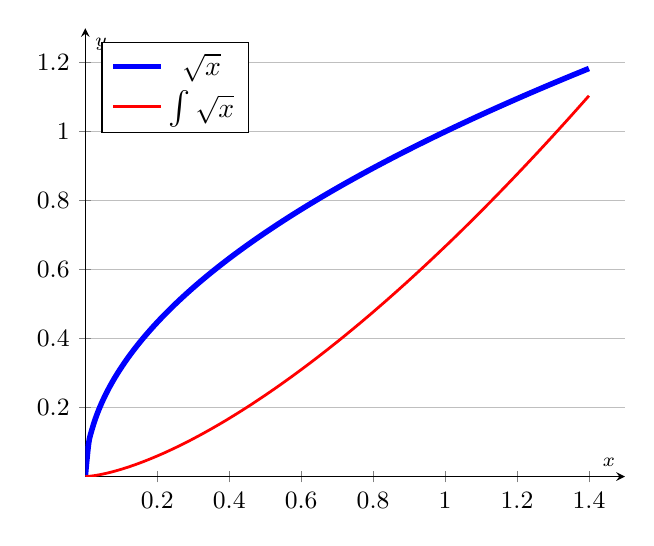
\begin{tikzpicture}[scale=1.0]
              \begin{axis}[axis lines=middle,xmin=0.0,xmax=1.5,ymin=0.0,ymax=1.3,legend pos=north west,ymajorgrids=true,
                xlabel=$\scriptstyle x$,
                ylabel=$\scriptstyle y$,
                tick label style={font=\small}]
                \addplot[no marks,domain=0.0:1.4,samples=150,smooth,line width=2pt,blue]{sqrt(x)};
                \addlegendentry{$\sqrt{x}$}
                \addplot[no marks,domain=0.0:1.4,samples=150,smooth,line width=1pt,red]{(2/3) * x^(3/2)};
                \addlegendentry{$\bigintssss \sqrt{x}$}
              \end{axis}
            \end{tikzpicture}
        \end{center}

    \noindent \textbf{Tétel.} Folytonos függvénynek van primitív függvénye, pontosabban Ha $f(x)$ folytonos az $[a,b]$ zárt intervallumon, akkor van olyan $F(x)$ függvény, amelyik folytonos az $[a,b]$-n és primitív függvény $(a,b)$-n.\\

    \paragraph*{Alapintegrálok}

    \noindent Azokat az integrálokat, amelyek valamilyen elemi függvény deriválásának megfordításakor keletkeznek, elemi integráloknak nevezzük.\\
    \renewcommand{\arraystretch}{2}
    \noindent $\begin{array}{ll}
        \bigintss x^n\ dx = \ddfrac{x^{n+1}}{n+1}$,\ ahol $n \neq -1,\ \text{speciálisan:}\ \bigintss 1 d x = x & \\
        \bigintss \ddfrac{1}{x}\ dx = \ln |x| & \bigintss x^{\alpha}\ dx = \ddfrac{1}{\alpha + 1}x^{\alpha + 1},\ \alpha \neq 1 \\
        \bigintss a^x\ dx = \ddfrac{1}{\ln a} a^x \ln a,\ \text{ahol}\ a > 0,\ a \neq 1 & \bigintss e^{x}\ dx = e^{x} \\
        \bigintss \sin{x}\ dx\ = -\cos x & \bigintss \cos x\ dx = \sin x \\
%        \bigintss \ddfrac{1}{\cos^2x}\ dx = \tan x & \bigintss \ddfrac{1}{\sin^2x}\ dx = -\cot x \\
%        \bigintss \ch x\ dx = \sh x & \bigintss \sh x\ dx = \ch x \\
%        \bigintsss \ddfrac{1}{\cosh^2x}\ dx = \tanh x & \bigintsss \ddfrac{1}{\sinh^2x}\ dx = -\coth x \\
%        \bigintsss \ddfrac{1}{\sqrt{1 - x^2}}\ dx = \arcsin{x} & \bigintsss \ddfrac{1}{\sqrt{1 + x^2}}\ dx = \arcsinh{x} \\
%        \bigintsss \ddfrac{1}{\sqrt{x^2 - 1}}\ dx = \arccosh x &
    \end{array}$\\
    \renewcommand{\arraystretch}{1}

    \subsection*{Integrálási szabályok}

    \paragraph*{Műveleti szabályok}

    \begin{itemize}
      \item Összeget és különbséget lehet tagonként integrálni, tehát:
      \[
        \bigintssss f = F,\ \bigintssss g = G \Longrightarrow \bigintssss \big[f \pm g \big] = F + G
      \]
      \item A konstansszorzó az integrál elé kiemelhető, azaz tetszőleges $c$ esetén:
      \[
        \bigintssss c \cdot f = c \bigintssss f
      \]
      \item \emph{Lineáris helyettesítés}. $f(ax + b)$ alakú integrandus $a, b \in \mathbb{R},\ a \neq 0$ és $F$ egy primitív függvénye $f$-nek:
      \[
        \bigintssss f(ax + b)dx = \ddfrac{F(ax + b)}{a}
      \]
      Példa:
      \[
        \bigintssss \sin (3x - 4)dx = \ddfrac{-cos(3x - 4)}{3}
      \]
      \item \emph{Helyettesítés hatványfüggvénybe}. $f^{(n)}(x)f'(x)$ alakú integrandus: ($n \neq 1$)
      \[
        \bigintssss f^{(n)}(x)f'(x) dx = \ddfrac{f^{(n+1)}(x)}{n+1}
      \]
      Példa:
      \[
        \bigintssss {(2x^2+5)4x}\ dx = \ddfrac{(2x^2+5)^6}{6}
      \]
      \item $\ddfrac{f'(x)}{f(x)}$ alakú integrandus:
      \[
        \bigintssss \ddfrac{f'(x)}{f(x)} dx = \left\{ \begin{array}{cc}
                                                 \ln f(x): & I \subseteq \Big\{x: f(x) > 0\Big\} \\
                                                 \ln(-f(x)): & J \subseteq  \Big\{x: f(x) < 0\Big\}
                                               \end{array}
        \right.
      \]
      \emph{Megjegyzés}: Itt \emph{I} és \emph{J} intervallum, a továbbiakban a fenti értelemben használjuk az $\bigintss \ddfrac{f'(x)}{f(x)} dx = \ln \Big|f(x)\Big|$ jelölést.\\
      \ \\
      Például:
      \[
        \bigintssss \ddfrac{2^x}{2^x-3} dx = \ddfrac{1}{\ln 2}\ln\Big|2^x-3\Big|
      \]
    \end{itemize}
				
    \subsection*{Határozott integrál}

    \noindent A gyakorlati életben, amikor konkrét integrálok kiszámítására van szükségünk, főként határozott integrálokat számolunk.
    \noindent Néhány, a határozott integrál fogalmára vezető probléma.

    \begin{itemize}
        \item A függvénygrafikon alatti terület.
        \item A munka értelmezése és kiszámítása.
        \item A nyomóerő meghatározása.\\
    \end{itemize}

    \paragraph*{Riemann-integrál}

    {\footnotesize \noindent {\color{blue} \faLightbulbO\ $\triangleright$ } }
    {\footnotesize\\
    \noindent Ismert, hogy az $u > 0$, $v > 0$ oldalú téglalap területe $u\cdot v$. Állapodjunk meg abban, hogy ha $u > 0$ és $v < 0$, akkor $u\cdot v$ a téglalap „előjeles területe” legyen.\\  Nézzük meg mi is az, hogy a
    \[
        H := \Big\{(x, y)\ \big|\ x \in [0, 1], y \in [0, x^2]\Big\}
    \]
    „parabola alatti tartománynak” mi lehet a területe.

    \noindent Osszuk fel a $[0, 1]$ intervallumot $n$ egyenlő részre. Az osztópontok
    \[
        x_0 = 0,\ x_1 = \ddfrac{1}{n},\ x_2 = \ddfrac{2}{n},\ \ldots,\ x_n = \ddfrac{n}{n}.
    \]
    Legyen $S_n := \ddfrac{1}{n} \cdot \Big(\dfrac{1}{n}\Big)^2 + \ddfrac{1}{n} \cdot \Big(\ddfrac{2}{n}\Big)^2 + \ldots + \ddfrac{1}{n} \cdot \Big(\ddfrac{n}{n}\Big)^n$, azaz olyan téglalapok területének az összege, amelyeknek az alapja $\ddfrac{1}{n}$, a magassága pedig az $id^2$ függvény osztópontokban vett függvényértéke ($\ref{fig:intsqr}$. ábra).\\

    \begin{figure}[H]
    	\centering
        \begin{center}
            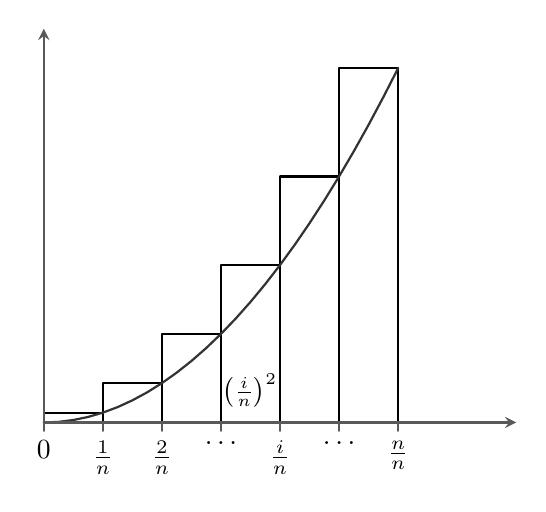
\begin{tikzpicture}[x=1.5cm,line cap=round, line join=round]
            \foreach \k [count=\z] in {1/2}
            {
                \begin{scope}[shift=(0:\z)]
                    \path [plot fill] plot [domain=0:2] (\x,{y(\x)}) -| cycle;
                    \foreach \x in {0, 1/2, 1, 3/2, 2, 5/2}
                       \path [bar,draw=black,fill=white]  (\x,0) |- (\x+1/2, {y((\x+\k))/2}) |- cycle;
                    \path [plot]  plot [domain=0:3] (\x,{y(\x)/2});
                    \path [axis] (0,5.0) |- (4.0,0);
                    \foreach \t [count=\x from 0] in {0,\frac{1}{n},\frac{2}{n},\ldots,\frac{i}{n},\ldots,\frac{n}{n}}
                        \path [axis, -] (\x/2,0) -- ++(0,-3pt) node [below] {$\t$};
                    \draw (2.6175cm,2pt) node[above]
                        {\small $\big(\frac{i}{n}\big)^2$};
                \end{scope}
            }
            \end{tikzpicture}
        \end{center}
        \caption{}
        \label{fig:intsqr}
    \end{figure}

    \noindent $S_n$ egy „lépcsősidom” területe. Ha növeljük az $n$ osztópontszámot, akkor a lépcsősidomok egyre jobban illeszkednek a $H$ halmazhoz, így elvárható, hogy az $\big(S_n\big)$ sorozat határértéke éppen a $H$ halmaz területe legyen.\\
    Felhasználva, hogy minden $k \in N$ esetén $1^2 + 2^2 + \ldots + k^2 = \ddfrac{k(k+1)(2k+1)}{6}$,
    \begin{center}
        $\lim S_n = \lim\ddfrac{1}{n^3} (1^2 + 2^2 + \ldots + n^2) = \lim \ddfrac{1}{n^3}\ddfrac{n(n + 1)(2n + 1)}{6}=$\\
        $\lim \ddfrac{2n^2 + 3n + 1}{6n^2} = \lim\ddfrac{2 + \ddfrac{3}{n} + \ddfrac{1}{n^2}}{6}=\ddfrac{1}{3}$
    \end{center}
    \noindent Legyen tehát a $H$ halmaz területe $\ddfrac{1}{3}$.\\

    \noindent Ezt a gondolatmenetet általánosítjuk.
    $\triangleleft$ \faLightbulbO}\\

    \noindent Legyen $f : [a, b] \to \mathbb{R}$ függvény.
    Legyen
    \[
        \tau := x_0, x_1, x_2, \ldots, , x_i, \ldots, x_n \subset [a, b],
    \]
    ahol
    \[
        a = x_0 < x_1 < x_2 < \ldots < x_{i-1} < x_i < \ldots < x_n = b
    \]
    az $[a,b]$ intervallum egy felosztása.\\

    \noindent Minden $[x_i-1, x_i]$ intervallumban vegyük fel egy $\xi_i$ pontot (i=1,2,\ldots,n). \\

    \noindent Készítsük el az $f$ függvény $\tau$ felosztáshoz tartozó közelítő összegét:
    \[
        \sigma(\tau) := f(\xi_1)(x_1-x_0)+f(\xi_2)(x_2-x_1)+ \ldots + f(\xi_n)(x_n-x_{n-1}) = \sum\limits_{i=1}^{n} f(\xi_i)(x_i-x_{i-1}).
    \]

    \noindent (Ez a $\sigma(\tau)$ felel meg a bevezető példa $S_n$ lépcsősidom területének, ott a $\xi_i$ pontot mindig az intervallum jobb szélén vettük fel.)\\
    Akkor mondjuk a függvényt integrálhatónak, ha a $\sigma(\tau)$ közelítő összegek „finomodó” felosztások során tetszőlegesen közel kerülnek egy számhoz. Pontosabban:\\

    \noindent \textbf{Definíció}. Azt mondjuk, hogy az $f : [a, b] \to \mathbb{R}$ függvény integrálható az $[a,b]$ intervallumon, ha van olyan $I \in \mathbb{R}$ szám, hogy bármilyen $\varepsilon > 0$ hibakorláthoz van olyan $\delta > 0$, hogy az $[a, b]$ intervallum minden olyan $\tau$ felosztására, amelyben
    \[
        \max \Big\{x_{i} - x_{i-1} \big| i = 1, 2, \ldots, n\Big\} < \delta
    \]
    és a $\tau$ felosztáshoz tartozó $[x_{i-1},\ x_i]$ intervallumokban vett tetszőleges $\xi_{i} \in [x_{i-1},\ x_i]$ pontok esetén a
    \[
        \sigma(\tau) = \sum\limits_{i=1}^{n} f(\xi_{i})(x_i - x_{i-1})
    \]
    közelítő összegre
    \[
        \big| \sigma(\tau) -I \big| < \varepsilon
    \]
    Ha $f$ integrálható az $[a, b]$ intervallumon, akkor ezt $f \in  R[a, b]$ jelölje (Riemann tiszteletére, aki az integrált ilyen módon bevezette), és legyen
    \[
        \bigintssss\limits_{a}^{b} f := I.
    \]
    („integrál a-tól b-ig”). Továbbá ekkor azt mondjuk, hogy a
    \[
        H := \Big\{(x, y)\ \big|\ x \in [a, b],\ \begin{array}{rc}
                                                 y \in [0, f(x)],\ \text{ha}\ &f(x) \geq 0 \\
                                                 y \in [f(x), 0],\ \text{ha}\ &f(x) < 0
                                               \end{array}
        \Big\}
    \]
    halmaznak („görbe alatti tartomány”) van előjeles területe, és ez a terület az $I \in \mathbb{R}$ szám.
    Röviden úgy szoktak hivatkozni erre a fogalomra, hogy bevezetve a $\Delta x_i := x_{i} - x_{i-1}$ jelölést,
    \[
        \lim\limits_{\Delta x_i \to 0}^{} f(\xi_{i}) \Delta x_{i} = I
    \]
    vagy
    \[
        \lim\limits_{\Delta x \to 0}^{} \sum f(\xi) \Delta x = \bigintssss\limits_{a}^{b} f(x)dx.
    \]

    {\footnotesize \noindent {\color{blue} \faLightbulbO\ $\triangleright$ } }
    {\footnotesize
    \noindent Könnyű látni, hogy ha $f : [a, b] \to \mathbb{R}$, $f(x) = c$ egy konstans függvény, akkor
    \[
        \lim\limits_{x_{i} \to 0}^{} f(\xi_{i}) \Delta x_{i} = \lim\limits_{\Delta x_{i} \to 0}^{} \sum\limits_{i=1}^{n} c(x_{i} - x_{i-1}) = c(b-a),
    \]
    amint ezt a szemlélet alapján is vártuk, tehát $f \in R[a, b]$ és $\bigintssss\limits_{a}^{b} f = c(b-a)$.
    $\triangleleft$ \faLightbulbO}\\

    \paragraph*{Az integrálhatóság feltételei}

    \noindent Legyen $f:[a,b] \to \mathbb{R}$ korlátos és $\tau$ egy felosztása $[a,b]$-nek. Az
    \[
        \omega(f, \tau) = S(f, \tau) - s(f, \tau)
    \]
    valós számot az $f$ függvény $\tau$-hoz tartozó \textbf{\emph{oszcillációs összeg}}ének nevezzük.\\

    \noindent \emph{Riemann-kritérium}: Egy $f:[a,b] \to \mathbb{R}$ korlátos függvény akkor és csak akkor Riemann-integrálható, ha $\forall \varepsilon > 0$ számhoz $\exists \tau$ felosztása $[a,b]$-nek úgy, hogy $\omega(f, \tau) < \varepsilon$.\\

    \noindent \textbf{Tétel}. Ha $f:[a,b] \to \mathbb{R}$ folytonos függvény, akkor $f$ Riemann-integrálható ($f \in R[a,b]$).\\

    \noindent \textbf{Tétel}. Ha $f:[a,b] \to \mathbb{R}$ monoton függvény, akkor $f$ Riemann-integrálható ($f \in R[a,b]$).\\

    \subsubsection*{A Riemann-integrál és a műveletek kapcsolata}

    \noindent Ha $f \in \mathcal{C}[a,b]$, akkor $f \in R[a,b]$. Ha $f \in R[a,b]$ és $f \in R[b,c]$, akkor $f \in R[a,c]$, sőt
    \[
        \bigintssss\limits_{a}^{b} f + \bigintssss\limits_{b}^{c} f  = \bigintssss\limits_{a}^{c} f
    \]

    \noindent Tehát az integrálási intervallum részekre bontásával az eredeti integrál a részeken vett integrálok összegével egyezik meg.\\

    \noindent Ha $f \in R[a,b]$ és $\lambda \in \mathbb{R}$, akkor $\lambda \in R[a,b]$, és
    \[
        \bigintssss\limits_{a}^{b} \lambda f = \lambda \bigintssss\limits_{a}^{b} f
    \]

    \noindent Ha $f,g \in R[a,b]$, akkor $f + g \in R[a,b]$, és
    \[
        \bigintssss\limits_{a}^{b} (f + g) = \bigintssss\limits_{a}^{b} f + \bigintssss\limits_{a}^{b} g
    \]

    \noindent Ha $f,g \in R[a,b]$, akkor $f \cdot g \in R[a,b]$. Nincs rá általános képlet.\\

    \noindent Ha $f,g \in R[a,b]$, és $f(x) \geq g(x)\ \forall x \in [a,b]$, akkor
    \[
        \bigintssss\limits_{a}^{b} f \geq \bigintssss\limits_{a}^{b} g
    \]

    \noindent Ha $f \in R[a,b]$, akkor
    \[
        \left|\bigintssss\limits_{a}^{b} f\right| \leq \bigintssss\limits_{a}^{b} |f|
    \]

    \noindent A határok felcserélésével előjelváltás történik.
    \[
        \bigintssss_{a}^{b}f(x)dx = -\bigintssss_{b}^{a}f(x)dx
    \]

	\section*{Newton-Leibniz-formula}
		
    \noindent A határozott és a határozatlan integrál kapcsolatát a Newton-Leibniz formula adja meg:
    \noindent Legyen $f:[a,b] \to \mathbb{R}\ $ Riemann integrálható és $F:[a,b] \to \mathbb{R}$ folytonos függvény úgy, hogy $\forall x \in (a,b)$-re az $F$ differenciálható $x$-ben és $F'(x) = f(x)$. Ekkor
    \[
        \bigintss_{a}^{b}f(x)dx := F(b) - F(a)
    \]
    \noindent Jelölés: $F(b) - F(a) = \Big[F(x)\Big]_{a}^{b}$. Így tehát a határozott integrál kiszámolásához is lényegében primitív függvényt kell keresnünk, ezért a határozatlan integrál esetében látott szabályok és módszerek itt is érvényben maradnak.\\

    \subsection*{Parciális intergrálás}

    \noindent A parciális integrálás egy igen fontos módszer, mert segítségével szorzat alakban megadott (vagy olyanná alakítható) integrandusok nagyrészét kiszámíthatjuk. Maga a módszer a szorzat függvény deriválási szabályából adódik:
    \[
        \bigintssss fg' = fg - \bigintssss f'g
    \]

    \noindent Az ötlet tehát, hogy a szorzat alakban megadott függvény egyik tényezőjét f-nek, másik tényezőjét $g \textquotesingle$-nek választva átírjuk az integrált. A megfelelő megválasztás alapja, hogy $f \textquotesingle g$-t könnyebben lehet integrálni mint $fg \textquotesingle$-t.

    \noindent Nem mindegy azonban, hogy melyik függvényt választjuk $f$-nek, illetve $g$-nek.\\

    \paragraph*{Parciális integrálás határozott esetben\\}

    Legyen $ f,g:[a,b] \to \mathbb{R}$ függvények az $[a,b]$ intervallumon differenciálhatók, és deriváltfüggvényük is folytonos.\\
    Ekkor az $f \cdot g' + f' \cdot g$ is folytonos, és $(f \cdot g)' = f' \cdot g + f \cdot g'$-t figyelembe véve a Newton-Leibniz-formula alapján
    \[
        \bigintssss\limits_{a}^{b} \Big(f'(x)g(x) + f(x)g'(x)\Big)dx = f(b)g(b) - f(a)g(a)
    \]
    átrendezve azt kapjuk, hogy
    \[
        \bigintssss\limits_{a}^{b} f'(x)g(x) = f(b)g(b) - f(a)g(a) - \bigintssss\limits_{a}^{b}f(x)g'(x) dx
    \]

    \noindent Természetesen ezt akkor tudjuk alkalmazni, ha a jobb oldalon álló integrál kiszámolható.\\

	\paragraph*{Helyettesítéses integrálás}

    \noindent A helyettesítéses integrálás módszere nagyon sokszor segítségünkre lehet a legkülönfélébb estekben is. Lényege, hogy az integrandusban valamilyen kifejezést helyettesítünk egy új változóval, ez által egy könnyebben integrálható kifejezést kapunk, amit kiintegrálunk, majd a végén visszahelyettesítjük az eredeti kifejezést.\\

    \noindent Az eljárás lényege tehát a következő:
    Legyen $g(x) = t$, ekkor $g'(x) = \ddfrac{dt}{dx}$, és ezért $g'(x) dx = dt$, vagyis:
    \[
        \bigintssss f(g(x))g\textquotesingle (x) dx = \bigintssss f(t) dt = F(t) = F(g(x))
    \]
    \noindent Példa:
    \[
        \bigintssss \ddfrac{3}{\cos^{2}(2x-3)} dx = \bigintssss \ddfrac{3}{\cos^{2}t}\ddfrac{dt}{2} = \ddfrac{3}{2} \tan t = \ddfrac{3}{2}\tan (2x-3)
    \]

    \paragraph*{Harározott esetben}
    \[
        \bigintssss\limits_{a}^{b} f(g(x))g\textquotesingle (x) dx = \bigintssss\limits_{g(a)}^{g(b)} f(t) dt = [F(t)]_{g(a)}^{g(b)}
    \]

    \noindent Példa: Határozzuk meg az egység sugarú (negyed-)kör területét.

    \noindent Az origó középpontú 1 sugarú kör egyenlete: $x^2 + y^2 = 1$, ezért az első síknegyedet választva az explicit függvénykapcsolatot az $y = \sqrt{1 - x^2}$ képlet írja le. A meghatározandó integrál tehát: $\bigintssss\limits_{0}^{1} \sqrt{1 - x^2} dx$.\\
    Alkalmazzuk az $x = \sin{y}$ helyettesítést $\Rightarrow dy = \ddfrac{1}{\sqrt{1- x^2}}dx$
    \[
        \bigintssss\limits_{0}^{1} \sqrt{1 - x^2} dx = \bigintssss\limits_{0}^{\ddfrac{\pi}{2}} 1 - \sin^{2}(y) dy = \bigintssss\limits_{0}^{\ddfrac{\pi}{2}} \cos^{2}(y) dx = \ddfrac{1}{2} \bigintssss\limits_{0}^{\ddfrac{\pi}{2}} 1 + \cos(2y) dy = \ddfrac{1}{2}\Big[y + \ddfrac{\sin(2y)}{2}\Big]_{0}^{\ddfrac{\pi}{2}} = \ddfrac{\pi}{4}
    \]

    \paragraph*{Integrálszámítás alkalmazása}

    \begin{itemize}
        \item Függvények alatti terület kiszámítása
        \item Síkidomok területének kiszámítása
        \item Forgástestek felszínének kiszámítása
        \item $R^{n}$-beli görbék ívhosszának kiszámítása
    \end{itemize}

%	\section*{A kezdeti érték probléma}
%		\begin{description}
%			\item[Differenciál egyenlet] \hfill \\
%				$ 0 < n \in \mathbb{N}, \ I \subset \R$ nyílt intervallum, \\
%				$ \Omega := I_1 \times \ldots \times I_n \subset \R^n$, ahol $ I_1,\ldots,I_n \subset \R$ nyílt intervallum \\
%				$f:I\times\Omega \rightarrow \R^n, \ f \in C $
				
%				Határozzuk meg a $ \varphi \in I \rightarrow \Omega$ függvényt úgy, hogy:
%				\begin{itemize}
%					\item $ D_{\varphi} $ nyílt intervallum
%					\item $ \varphi \in D $
%					\item $ \varphi'(x) = f(x, \varphi(x)) \quad (x \in D_{\varphi}) $
%				\end{itemize}
%				
%				Ezt a feladatot nevezzük differenciálegyenletnek.
%			\item[Kezdeti érték probléma] \hfill \\
%				Ha az előzőekhez még adottak: $ \tau \in I$, és $ \xi \in \Omega$ \\
%				Illetve a $\varphi$ függvényre még teljesül:
%				\begin{itemize}
%					\item $\tau \in D_{\varphi}$ és $ \varphi(\tau) = \xi $
%				\end{itemize}
%				
%				Akkor kezdeti érték problémának (Cauchy feladatnak) nevezzük.
%		\end{description}
	
    \section*{Lineáris, ill. magasabb rendű lineáris differenciálegyenletek}

    \noindent Az olyan egyenleteket, melyben az ismeretlen függvény deriváltja, illetve deriváltjai szerepelnek, differenciál-egyenleteknek nevezzük. Tehát egy differenciálegyenletben szerepelhetnek:
    \begin{itemize}
        \item konstansok;
        \item egy vagy több független változó;
        \item az ismeretlen függvény, illetve függvények közönséges, illetve parciális deriváltja, illetve deriváltjai.
    \end{itemize}

    \paragraph*{Differenciálegyenletek osztályozása}

    \noindent Ha a differenciálegyenletben egyetlen független változó van, akkor a derivált közönséges derivált. Ebben az esetben \textbf{\emph{közönséges differenciálegyenlet}}ről beszélünk.\\

    \noindent Ha a differenciálegyenletben kettő vagy több független változó van, akkor a derivált parciális derivált. Ekkor a szóban forgó egyenlet egy \textbf{\emph{parciális differenciálegyenlet}}.\\

    \noindent Ha az ismeretlen függvények száma egynél több, akkor az ismeretlen függvények számával egyenlő számú differenciálegyenletből álló \textbf{\emph{differenciálegyenlet-rendszer}}rel van dolgunk.\\

    \noindent A \textbf{\emph{differenciálegyenlet rendje}} az egyenletben szereplő legmagasabb rendű derivált rangjával egyenlő.\\

    \noindent A közönséges differenciálegyenletek közül azokat, amelyekben az ismeretlen függvény és ennek a deriváltjai legfeljebb csak első hatványon fordulnak elő és szorzatuk nem szerepel, \textbf{\emph{lineáris differenciálegyenlet}}nek nevezzük. Ellenkező esetben \textbf{\emph{nemlineáris differenciálegyenlet}}ekről beszélünk.\\

    \noindent Ha a közönséges differenciálegyenletben van olyan tag, amely állandó, vagy amelyben csak a független változó szerepel, akkor a differenciálegyenlet \textbf{\emph{inhomogén differenciálegyenlet}}. Ellenkező esetben azt mondjuk, hogy a differenciálegyenlet \textbf{\emph{homogén differenciálegyenlet}}.\\

    \noindent Ha a közönséges differenciálegyenletben a függvényt és a deriváltjait tartalmazó tagok állandók, akkor az egyenletet \textbf{\emph{állandó együtthatós differenciálegyenlet}}nek nevezzük.  Ellenkező esetben \textbf{\emph{függvényegyütthatós differenciálegyenlet}}ről beszélünk.\\

    \noindent Egy $f$ függvényt a \textbf{\emph{differenciálegyenlet megoldásának}} nevezünk, ha deriváltjaival együtt azonosan kielégíti a differenciál-egyenletet.\\

    \noindent Egy $f$ függvényt  az n-edrendű  differenciálegyenlet \textbf{\emph{általános megoldásának}} nevezünk, ha deriváltjaival együtt azonosan kielégíti a differenciálegyenletet és pontosan $n$ db egymástól függetlenül megválasztható szabad paramétert tartalmaz.\\

    \noindent Egy $f$ függvényt az n-edrendű differenciálegyenlet \textbf{\emph{partikuláris megoldásának}} nevezünk, ha deriváltjaival együtt azonosan kielégíti a differenciálegyenletet és legfeljebb $n-1$ db egymástól függetlenül megválasztható szabad paramétert tartalmaz.\\

    \noindent \emph{Megjegyzés}: A szabad paraméterek helyébe egy-egy (valós) számot helyettesítve a differenciálegyenlet valamely megoldását kapjuk.\\

    \noindent Adott egy $D \subset \mathbb{R} \times \mathbb{R}^{n}\ (n \in \mathbb{N})$ tartomány és $f:D \to \mathbb{R}^n$ folytonos függvény.\\

    \noindent Keresünk: $I \subset \mathbb{R}$ nyílt intervallumot és $\varphi: I \to \mathbb{R}^n$ differenciálható függvényt, amelyre
    \begin{itemize}
      \item $(t, \varphi(t)) \in D\qquad (\forall t \in I)$
      \item $\varphi'(t) = f(t, \varphi(t))\qquad (\forall t \in I)$
    \end{itemize}

    \noindent Ezt a feladatot explicit \textbf{\emph{elsőrendő közönséges differenciálegyenletnek}} nevezzük.\\


    \noindent Jelölése:
    \begin{equation} \label{eu_eq1}
        x'(t) = f(t, x(t)) \qquad \text{vagy}\ \qquad x' = f \circ (id, x)
    \end{equation}

    \noindent Ha ilyen $I$ intervallum és $\varphi$ függvény létezik, akkor azt mondjuk, hogy a $\varphi$ az $(1)$ \textbf{\emph{differenciálegyenlet megoldása}} $I$-n.
\newpage
    \subsubsection*{Kezdetiérték probléma}

    Legyen $D \subset \mathbb{R} \times \mathbb{R}^{n}\ (n \in \mathbb{N})$ tartomány és $f:D \to \mathbb{R}^{n}$ folytonos függvény, $(p_1, p_2) \in D \subset \mathbb{R} \times \mathbb{R}^{n}$ pedig tetszőleges pont. A $\varphi: I \to \mathbb{R}^n$ differenciálható függvény az
    \begin{equation} \label{eu_eq2}
        x' = f(t, x(t)), \qquad x(p_1) = p_2
    \end{equation}
    \emph{kezdetiérték-probléma} egy megoldása, ha
    \begin{itemize}
      \item $\varphi$ az $x' = f(t, x(t))$ differenciálegyenlet egy megoldása $I$-n,
      \item $p_1 \in I$
      \item $\varphi(p_1) = p_2$
    \end{itemize}

    \noindent Továbbiakban kezdetiérték-probléma = K.É.P.

    \paragraph*{Kezdeti érték megoldására vonatkozó kérdések}

    \begin{enumerate}
      \item A megoldás létezése
      \item A megoldások egyértelműsége
      \item A megoldások előállítása
      \begin{itemize}
        \item pontos megoldás (megoldóképlet)
        \item közelítő megoldás
      \end{itemize}
      \item A megoldások függése (például) a kezdeti értéktől
      \item Minőségi vizsgálatok: A megoldások bizonyos tulajdonságainak (például periodicitás) vizsgálata a differenciálegyenlet ismerete nélkül
    \end{enumerate}

    \paragraph*{A megoldás létezése}

    \noindent \textbf{Tétel}. (Cauchy-Peano-féle egzisztenciatétel): Tegyük fel, hogy a $D \subset \mathbb{R} \times \mathbb{R}^{n}\ (n \in \mathbb{N})$ tartományon értelmezett és $f:D \to \mathbb{R}^{n}$ függvény folytonos. Ekkor bármely $(p_1, p_2) \in D$ esetén az
    \[
        x' = f(t, x(t)), \qquad x(p_1) = p_2
    \]
    \emph{kezdetiérték problémának van megoldása}.

    \paragraph*{A megoldások egyértelműsége}

    \noindent A K.É.P globálisan \textbf{\emph{egyértelműen oldható meg}}, ha létezik olyan $\tilde{I} \subset \mathbb{R}$ nyílt intervallum és olyan $\tilde{\varphi}: \tilde{I} \to \mathbb{R}$ megoldása a kezdetiérték-problémának, hogy annak bármely más megoldása $\tilde{\varphi}$ egy leszűkítése. Ebben az esetben a $\tilde{\varphi}$ függvény a kezdetiérték-probléma \textbf{\emph{teljes megoldásának}} nevezzük.\\

    \noindent A K.É.P egy $\varphi^{*}: I^{*} \to \mathbb{R}^{n}$ megoldás \textbf{\emph{maximális megoldás}}, ha nincs olyan $\varphi^{*}$-től különböző megoldás, amelyiknek a leszűkítése $\varphi^{*}$ lenne. Ha $\varphi$ teljes megoldás $\Rightarrow$ $\varpi$ maximális megoldás is. (fordítva nem igaz).\\
\newpage
    \noindent Az K.É.P \textbf{\emph{lokálisan egyértelműen oldható meg}}, ha a $(p_1, p_2) \in \mathbb{R} \times \mathbb{R}^{n}$  pontnak létezik olyan $k(p_1, p_2) \subset \mathbb{R} \times \mathbb{R}^{n}$ környezete, hogy az $f$ függvényt erre leszűkítve a megfelelő K.É.P megoldása már globálisan egyértelmű.\\

    \noindent \textbf{Tétel}. Ha K.É.P minden $(p_1, p_2) \in D$ esetén lokálisan egyértelműen oldható meg, akkor minden K.É.P megoldása globálisan egyértelmű is.\\

    \noindent \textbf{Tétel}. (\emph{Picard–Lindelöf-féle egzisztencia\text{-} és unicitástétel}): Legyen $n \in \mathbb{N},\ D \subset \mathbb{R} \times \mathbb{R}^{n}$ egy tartomány és $(p_1, p_2) \in D$. Tegyük fel, hogy
    \begin{itemize}
      \item az $f: D \to \mathbb{R}^{n}$ függvény folytonos D-n
      \item az $f$ függvény a $(p_1, p_2)$ pontban a második változójában lokális Lipschitz-feltételeknek tesz eleget, azaz
      \begin{center}
        $\exists k(p_1, p_2) \subset D \qquad \text{és}\qquad L_{(p_1, p_2)} > 0$,\ \text{hogy}\\
        $\Vert f(t, \overline{u}) - f(t, \overline{\overline{u}})\Vert \leq L_{(p_1, p_2)}\Vert\overline{u} - \overline{\overline{u}}\Vert \qquad (\forall (t, \overline{u}),\ (t, \overline{\overline{u}}) \in k(p_1, p_2))$
      \end{center}
    \end{itemize}
    Ekkor a K.É.P létezik megoldása és az lokálisan (sőt globálisan) egyértelmű.\\

    \subsubsection*{Szétválasztható változójú (szeparábilis) differenciálegyenletek\\}

    \noindent Tegyük fel, hogy $I, J \in \mathbb{R}$ nyílt intervallum, $\Omega := I \times J$ és
    \[
        g: I \to \mathbb{R}, \quad h : J \to \mathbb{R}
    \]
    folytonos függvények. Ekkor az
    \begin{equation} \label{eu_eq3}
        x'(t) = g(t) h(x(t))\qquad \text{vagy}\qquad x' = g \cdot h \circ x
    \end{equation}
    feladatot \textbf{\emph{szétválasztható változójú}} (vagy \textbf{\emph{szeparábilis}}) differenciálegyenletnek nevezzük.\\

    \noindent Ha $(p_1, p_2) \in I \times J$, akkor az
    \begin{equation} \label{eu_eq4}
        x' = g(t)h(x(t)),\qquad x(p_1) = p_2
    \end{equation}
    feladat a (\ref{eu_eq3}) egyenletre vonatkozó \emph{\textbf{kezdetiérték-probléma}}.\\

    \noindent \emph{Megjegyzés}: Az elnevezés onnan ered, hogy az ilyen differenciálegyenletek átrendezhetők úgy, hogy az $y$ változó csak az egyik, az $x$ változó pedig csak a másik oldalon forduljon elő.\\

    \noindent Példa:\\

    \noindent $y' = \ddfrac{x^2 + x}{2y} \Rightarrow y1 = (x^2 + x) \cdot \ddfrac{1}{2y}$.\\
    \noindent $y'x + y' - y^2 + 2y = 0 \Rightarrow (y^2 - 2y)\cdot \ddfrac{1}{x+1}$.
\newpage
    \subsection*{Elsőrendű lineáris differenciálegyenletek}

    \noindent Tegyük fel, hogy $I \subset \mathbb{R}$ nyílt intervallum és $f,g: I \to \mathbb{R}$ folytonos függvények. Ekkor az
    \begin{equation}\label{eu_eq5}
      x'(t) + f(t)x(t) = g(t) \qquad (t \in I)
    \end{equation}
    feladatot elsőrendű lineáris differenciálegyenletnek nevezzük.\\

    \noindent Ha $(p_1, p_2) \in I \times \mathbb{R}$, akkor az
    \[
        x'(t) + f(t)x(t) = g(t), \qquad x(p_1) = p2 \qquad (t \in I)
    \]
    feladat az (\ref{eu_eq5}) egyenletre vonatkozó \textbf{\emph{kezdetiérték-probléma}}.\\

    \paragraph*{A feladat megoldása homogén-inhomogén módszerrel}

    \noindent Tekintsük először az
    \begin{equation}\label{eu_eq6}
      x' + f x = 0
    \end{equation}
    homogén lineáris differenciálegyenletet, amelynek általános megoldása
    \[
        \varphi(t) = c \cdot e^{-\bigintsss\limits_{a}^{t}f(s) ds} = c \cdot \varphi_0(t) \qquad (t \in I)
    \]
    alakú, ahol $a \in I$ rögzített pont és $c$ tetszőleges valós szám.\\

    \noindent Az
    \begin{equation}\label{eu_eq7}
        x' + f x = g
    \end{equation}
    inhomogén egyenletre a következő teljesül: ha $\psi_1$ és $\psi_2$ (\ref{eu_eq7}) megoldásai, akkor a $\psi := \psi_1 - \psi_2$ függvény kielégíti a (\ref{eu_eq6}) egyenletet.\\

    \noindent Ebből következik, hogy ha ismerjük az inhomogén egyenlet egy $\psi_p$ (partikuláris) megoldását, akkor (\ref{eu_eq7}) tetszőleges megoldása
    \[
        \psi = \varphi + \psi_p
    \]
    alakú, ahol $\varphi$ homogén egyenlet egy megoldása.\\

    \noindent Az előbbi megoldás a következő formában egyszerűbben megjegyezhető:
    \begin{center}
        \ovalbox{\makecell{inhomogén egyenlet \\ általános megoldása}} = \ovalbox{\makecell{homogén egyenlet \\ általános megoldása}} + \ovalbox{\makecell{az inhomogén egyenlet \\ egy partikuláris megoldása}}
    \end{center}

    \noindent Az inhomogén egyenlet egy partikuláris megoldását a Lagrange-tól eredő állandók variálásának a módszerével határozzuk meg.\\

    \noindent Tegyük fel, hogy $I \subset \mathbb{R}$ nyílt intervallum $f,g: I \in \mathbb{R}$ folytonos függvények és $(p1_, p_2) \in I \times \mathbb{R}$. Ekkor az
    \[
        x' + fx = g,\qquad x(p_1) = p_2
    \]
    kezdetiérték probléma globálisan egyértelműen oldható meg. A $\psi$ teljes megoldás értelmezési tartománya az egész $I$ intervallum, és a teljes megoldás
    \[
        \psi(t) = \xi \cdot \varphi_{0}(t) + \varphi_{0}(t) \bigintssss\limits_{p_1}^{t}(\varphi_{0}(s))^{-1}g(s) ds \qquad (t \in I)
    \]
    (ez a Cauchy-féle formula), ahol
    \[
        \varphi_{0}(t) := e^{\bigintssss\limits_{p_1}^{4}f(s) ds} \qquad (t \in I)
    \]
    a homogén egyenlet egy megoldása.\\

    \noindent Az $x' + fx = g$ inhomogén egyenlet megoldásai a
    \[
        \psi(t) = c\varphi_{0}(t) + \psi_{part}(t) = c\varphi_{0}(t) + \varphi_{0}(t)\bigintssss\limits_{p_1}^{t}(\varphi_{0}(s)) g(s) ds \qquad (t \in I,\ c \in \mathbb{R})
    \]
    függvények, illetve ezek leszűkítései.\\

    \noindent \textbf{Tétel}. (\emph{Szuperpozíció elve}): Tegyük fel, hogy $\psi_{1}$ megoldása az
    \[
        x' + fx = g_1
    \]
    egyenletnek, $\psi_2$ pedig megoldása az
    \[
        x' + fx = g_2
    \]
    egyenletnek, akkor $\psi_1 + \psi_2$ megoldása az
    \[
        x' + fx = g_1 + g_2
    \]
    egyenletnek.\\

    \paragraph*{n-ed rendű lineáris differenciálegyenletek}

    \noindent Legyen $n \in \mathbb{N},\ I \subset \mathbb{R}$ nyílt intervallum, és tegyük fel, hogy az $a_i: I \to \mathbb{R}$ $(i = 0,1, \ldots, n-1)$ és a $b:I \to \mathbb{R}$ függvények folytonosak. Ekkor az
    \[
        x^{(n)} + a_{n-1}x^{(n-1)} + \ldots + a_{1}x' + a_{0}x = b
    \]
    feladatot \emph{n}\textbf{\emph{-edrendű lineáris differenciálegyenletnek}} nevezzük. Ha $b \equiv 0$, akkor az egyenlet \textbf{\emph{homogén}}, az ellenkező esetben \textbf{\emph{inhomogén}}. \textbf{\emph{Állandó együtthatós}} az egyenlet, ha az $a_i\ (i = 0, 1, \ldots, n-1)$ együtthatók valós számok.\\

    \noindent Legyen $n \in \mathbb{R},\ I \subset \mathbb{R}$ nyílt intervallum, és tegyük fel, hogy az
    \[
        a_i : I \to \mathbb{R} \qquad (i = 0, 1, \ldots, n-1)\ \text{és a}\ b: I \to \mathbb{R}
    \]
    függvények folytonosak. Ha $p \in I$ és $s_1, s_2, \ldots, s_{n-1} \in \mathbb{R}$, akkor az
    \begin{center}
        $x^{(n)} + a_{n-1}x^{(n-1)} + \ldots + a_{1}x' + a_{0}x = b$\\
        $x(p) = s_0,\ \quad x'(p) = s_1,\ \ldots,\ x^{(n-1)}(p) = s_{n-1}$
    \end{center}
    feladatot az n-edrendű lineáris differenciálegyenletre vonatkozó \textbf{\emph{kezdetiérték-problémának}} nevezzük.\\

    \noindent \textbf{A megoldások létezése és egyértelműsége.} Az n-edrendű lineáris differenciálegyenletre vonatkozó tetszőleges kezdetiérték-probléma globálisan egyértelműen oldható meg, és minden teljes megoldás értelmezési tartománya az egész $I$ intervallum.\\
\newpage
    \noindent \textbf{A megoldáshalmaz szerkezet}
    \begin{itemize}
        \item A homogén n-endrendű lineáris differenciálegyenlet teljes megoldásainak az $\mathcal{M}_{h}$ halmaza n-dimenziós lineáris tér $\mathbb{R}$ felett.
        \item Legyen $\psi_{p}$ az \textbf{\emph{inhomogén}} n-edrendű lineáris differenciálegyenlet egy (partikuláris) megoldása. Ekkor az egyenlet tetszőleges megoldása
        \[
            \psi = \varphi + \psi_{part}
        \]
        alakú, ahol $\varphi$ a homogén egyenlet egy megoldása.
    \end{itemize}

    \noindent A homogén egyenlet $\mathcal{M}_{h}$ megoldáshalmazának egy bázisát a homogén egyenlet egy \textbf{\emph{alaprendszerének}} nevezzük.\\
    \begin{enumerate}
        \item megjegyzés: A fenti megoldás a következő formában egyszerűbben megjegyezhető:
        \begin{center}
            \ovalbox{\makecell{inhomogén egyenlet \\ általános megoldása}} = \ovalbox{\makecell{homogén egyenlet \\ általános megoldása}} + \ovalbox{\makecell{az inhomogén egyenlet \\ egy partikuláris megoldása}}
        \end{center}
        \item megjegyzés: Inhomogén egyenlet megoldásának előállításához tehát ismernünk kell
        \begin{itemize}
            \item a homogén egyenlet egy alaprendszerét és
            \item az inhomogén egyenlet egy partikuláris megoldását.
        \end{itemize}
    \end{enumerate}

    \noindent Az állandók variálásának a módszerével a homogén egyenlet alaprendszerének (n lineárisan független megoldásának) az ismeretében egy partikuláris megoldás már előállítható.\\

    \noindent Ez az jelenti, hogy inhomogén egyenlet megoldásához elegendő a homogén egyenlet egy alaprendszerét meghatározni. Az alaprendszer előállítására azonban csak az állandó együtthatós egyenletek esetében van általános módszer.\\

    \noindent \textbf{Az állandók variálásának a módszere}: Tekintsük az
    \[
        x^{(n)}(t) + a_{n-1}x^{(n-1)}(t) + \ldots + a_{0}x(t) = b(t) \qquad (t \in I)
    \]
    inhomogén egyenletet, valamint a neki megfelelő
    \[
        x^{(n)}(t) + a_{n-1}x^{(n-1)}(t) + \ldots + a_{0}x(t) = 0 \qquad (t \in I)
    \]
    homogén egyenletet.

    \noindent Legyen $\varphi_1, \varphi_2, \ldots, \varphi_n$ a homogén egyenlet egy alaprendszere. Ekkor az inhomogén egyenlet egy partikuláris megoldása előállítható a
    \[
        \psi_{p}(t) = c_1(t)\varphi_{1}(t) + \ldots + c_n(t)\varphi_{n}(t) \qquad (t \in I)
    \]
    alakban, ahol a $c'(t) := (c'_{1}(t), \ldots, c'_{n}(t))^{T}$ függvénynek a következő lineáris algebrai egyenletrendszer a megoldásai
    \begin{equation}\label{eu_eq8}
        \Phi(t) \cdot c'(t) = \begin{array}{c}
                                0 \\
                                0 \\
                                \vdots \\
                                b(t)
                              \end{array} \qquad (t \in I)
    \end{equation}
    ahol
    \[
        \Phi(t) := \left[ \begin{array}{ccc}
                     \varphi_1(t) & \ldots & \varphi_n(t) \\
                     \varphi'_1(t) & \vdots & \varphi'_n(t) \\
                     \vdots & \ddots & \vdots \\
                     \varphi_1^{n-1}(t) & \ldots & \varphi_n^{n-1}(t)
                   \end{array}\right] \qquad (t \in I)
    \]
    a Wronski-féle mátrix.\\

    \noindent \emph{Megjegyzés}: A $\psi_{p}$ partikuláris megoldás előállításához tehát először meg kell oldani a (\ref{eu_eq8}) lineáris algebrai egyenletrendszert a $c'_{1}(t), \ldots, c'_{n}$ ismeretlen függvényekre, amelyekből már integrálással előállíthatók a számukra szükséges $c_1(t), c_2(t), \ldots, c_{n}(t)\ (t \in \mathbb{R})$ függvények.\\

    \noindent \textbf{Tétel}. (\emph{Szuperpozíció elve}): Tegyük fel, hogy $\psi_{1}$ megoldása az
    \[
        x^{(n)}(t) + a_{n-1}x^{(n-1)}(t) + \ldots + a_{0}x(t) = b_1
    \]
    egyenletnek, $\psi_2$ pedig megoldása az
    \[
        x^{(n)}(t) + a_{n-1}x^{(n-1)}(t) + \ldots + a_{0}x(t) = b_2
    \]
    egyenletnek, akkor $\psi_1 + \psi_2$ megoldása az
    \[
        x^{(n)}(t) + a_{n-1}x^{(n-1)}(t) + \ldots + a_{0}x(t) = b_1 + b_2
    \]
    egyenletnek.\\

    \paragraph*{Az állandó együtthatós n-edrendű homogén lineáris differenciálegyenlet egy alaprendszerének az előállítása}

    \noindent Legyen $n \in \mathbb{N}$ és $a_0, a_1, \ldots, a_{n-1} \in \mathbb{R}$. Az
    \begin{equation}\label{eu_eq9}
        x^{(n)}(t) + a_{n-1}x^{(n-1)}(t) + \ldots + a_{0}x(t) = 0
    \end{equation}
    feladatot \emph{n}\textbf{\emph{-edrendű állandó együtthatós homogén lineáris differenciálegyenletnek}} nevezzük.\\

    \noindent \textbf{Tétel}. Tegyük fel, hogy az
    \begin{equation}\label{eu_eq10}
        x^{(n)} + a_{n-1}x^{(n-1)} + \ldots + a_{1}x' + a_{0}x = 0 \qquad (a_0, a_1, \ldots, a_{n-1} \in \mathbb{R})
    \end{equation}
    egyenlet
    \[
        K(z) = z^{n} + a_{n-1}z^{n-1} + \ldots + a_1z + a_0
    \]
    karakterisztikus polinomjának a $\lambda$ szám $m$-szeres gyöke. Ekkor
    \[
        \varphi_1(t) = e^{\lambda t},\ \varphi_2(t) = te^{\lambda t}, \ldots, \varphi_m(t) = t^{m-1}e^{\lambda t} \qquad (t \in \mathbb{R})
    \]
    függvények a (\ref{eu_eq10}) egyenlet lineárisan független valós megoldásai.

    \paragraph*{Az állandó együtthatós n-edrendű inhomogén lineáris differenciálegyenlet egy partikuláris megoldásának az előállítása}

    \noindent \emph{Megjegyzés}: Az
    \[
        x^{(n)}(t) + a_{n-1}x^{(n-1)}(t) + \ldots + a_{0}x(t) = b(t) \qquad (t \in I)
    \]
    állandó együtthatós n-edrendű inhomogén lineáris differenciálegyenlet egy partikuláris megoldásának az előállításához felhasználhatjuk az állandók variálásának a módszerét. Ez elvben mindig célhoz vezet, azonban esetenként meglehetősen fáradságos, sok számolást igénylő eljárás. Ezért "megbecsülendők" azok a módszerek, amelyek révén más úton juthatunk el egy partikuláris megoldáshoz. Egy ilyen módszer a próbafüggvény-módszer, amelyik bizonyos speciális jobboldal, vagyis b függvény esetén alkalmazható.\\

    \noindent \textbf{Tétel}. (\emph{Próbafüggvény-módszer}) Tekintsük az
    \[
        x^{(n)}(t) + a_{n-1}x^{(n-1)}(t) + \ldots + a_{0}x(t) = P(t)e^{\alpha t}\big(c \sin{(\beta t)} + d \cos (\beta t)\big) \qquad (t \in \mathbb{R})
    \]
    egyenletet, ahol $a_0, a_1, \ldots, a_{n-1};c;d;\alpha;\beta$ valós számok és $P$ egy polinom.\\

    \noindent Legyen $\mu := \alpha + i\beta$ és\\
    $\tilde{k} := \left\{\begin{array}{cl}
                    0, & \text{ha}\ \mu\ \text{nem gyöke a homogén egyenletrendszer karakterisztikus polinomjának}\\
                    k, & \text{ha}\ \mu\ \text{\emph{k}-szoros gyöke a homogén egyenletrendszer karakterisztikus polinomjának}
                  \end{array}\right.
    $

    \noindent Ekkor az egyenletnek létezik
    \[
        \psi_{p}(t) = t^{\tilde{k}}G(t) \cdot e^{\alpha t}\big(A \sin(\beta t) + B \cos (\beta t)\big)
    \]
    alakú megoldása, ahol $A, B \in \mathbb{R}$ és $G$ egy legfelejebb  $deg(P)$-edfokú polinom.

%    \paragraph*{n-ed rendű lineáris differenciálegyenletek}

%    \noindent Legyen $n \in \mathbb{N},\ I \subset \mathbb{R}$ nyílt intervallum, és tegyük fel, hogy az $a_i : I \to \mathbb{R}\ (i = 0,1,\ldots, n-1)$ és a $b: I \to \mathbb{R}$ függvények folytonosak. Ekkor az
%    \[
%        x(n) + a_{n-1}x(n-1) + \ldots + a_1x' + a_0x = b
%    \]
%    feladatot $n$-edrendű lineáris differenciálegyenletnek nevezzük. Ha $b \equiv 0$, akkor az egyenlet homogén, ellenkező esetben inhomogén. Állandó együtthatós az egyenlet, ha az $a_i\ (i = 0,1,\ldots,n-1)$ együtthatók valós számok.\\

%    \section*{Lin diff egyenletek másképp}

%	\subsection*{Lineáris differenciálegyenletek}

%    \noindent Legyen $y$ az ismeretlen $g$ és $h$ pedig ismert egyváltozós függvények. Ekkor az
%    \[
%        y' + g(x)y = h(x)
%    \]
%    alakra hozható differenciálegyenletet \textbf{\emph{elsőrendű lineáris differenciálegyenlet}}nek nevezzük.\\

%    \noindent Például:
%    \begin{itemize}
%        \item $y' + (x-2)y = x^2 -3x + 16$\ -\ \text{lineáris}
%        \item $y' + 2y^2 = x^3 - 1$\ -\ \text{nem lineáris}
%    \end{itemize}

%    \noindent Legyen $y$ az ismeretlen $f$ és $g$ pedig ismert egyváltozós függvények. Ekkor az
%    \[
%        y' = f(x)g(y)
%    \]
%    alakra hozható differenciálegyenletet \textbf{\emph{szétválasztható változójú differenciálegyenlet}}nek nevezzük.\\


%    \noindent Az \emph{elsőrendű lineáris differenciálegyenlet} \emph{\textbf{homogén}}, ha a következő alakra hozható.
%    \[
%        y' + g(x)y = 0 \qquad (\text{azaz}\ h\ \text{zavaró függvény} \equiv 0)
%    \]

%    \noindent \emph{Megjegyzés}: A lineáris jelző arra utal, hogy $y$ és $y'$ mindegyike csak első hatványon szerepel a differenciálegyenletben.\\

%    \noindent Az elsőrendű lineáris differenciálegyenlet állandó együtthatójú, ha a differenciálegyenlet
%    \[
%        y' + g(x)y = h(x)
%    \]
%    alakjában a $g(x)$ függvény konstans, azaz az egyenlet a következő alakú
%    \[
%        y' + ky = h(x)
%    \]

%    \noindent \textbf{Tétel}. Az $y' + ky = 0$ elsőrendű állandó együtthatós lineáris homogén differenciálegyenlet általános megoldása:
%    \[
%        y = Ce^{-kx}
%    \]

%    \noindent ---------------------
%			\begin{description}
%				\item[Definíció] \hfill \\
%				A lineáris differenciálegyenlet olyan differenciálegyenlet, melyre:\\
%					$ n=1, \quad I,I_1 \subset \R $ nyílt intervallumok, $f:I\times I_1 \rightarrow \R$, ahol \\
%					$g,h : I \rightarrow \R, \ g,h \in C, \ I_1 := \R$ és \\
%					$f(x,y) := g(x)\cdot y + h(x) \quad (x \in I, y \in I_1 = \R) $\\
%					$ \Rightarrow \varphi'(x) = f(x, \varphi(x)) = g(x) \cdot \varphi(x) + h(x) \quad (x \in D_{\varphi})$
%				\item[Homogenitás] \hfill \\
%					A lineáris differenciálegyenlet homogén ha $ h \equiv 0$ (különben inhomogén)
%				\item[Kezdeti érték probléma] \hfill
%				\begin{itemize}
%					\item Minden lineáris differenciálegyenletre vonatkozó kezdeti érték probléma megoldható és \\
%					$\forall \varphi, \psi $ megoldásokra: $ \varphi(t) = \psi(t) \quad (t \in D_{\varphi} \cap D_{\psi} )$
%					\item Minden homogén lineáris differenciálegyenlet ($\varphi : I \rightarrow \R$) megoldása a következő alakú: \\
%					$ c\varphi_0$, ahol \\
%					 $c \in \R$ és $\varphi_0(t) = e^{G(t)} \quad (G:I\rightarrow\R, \ G \in D, $ és $ G' = g)$
%					\item Állandók variálásának módszere:\\
%					$ \exists m:I\rightarrow\R, \ m \in D : m\cdot\varphi_0$ megoldása az (inhomogén) lineáris differenciálegyenletnek
%					\item Partikuláris megoldás: \\
%					$M := \Big\{ \varphi : I \rightarrow \R : \varphi'(t) = g(t)\cdot\varphi(t) + h(t) \ (t \in I)\Big\} $ \\
%					$M_h := \Big\{ \varphi : I \rightarrow \R : \varphi'(t) = g(t)\cdot\varphi(t) \ (t \in I)\Big\} $\\
%					$\Rightarrow \forall \psi \in M : M = \psi + M_h = \Big\{\varphi + \psi : \varphi \in M_h\Big\}$\\
%					(És itt $\psi$ az előzőek alapján $m\cdot\varphi_0$ alakban írható)
%					\item Példa: Radioaktív bomlás: \\
%					$ m_0 > 0$ - kezdeti anyagmennyiség \\
%					$ m \in \R \rightarrow \R $ - tömeg-idő függvénye, ahol \\
%					$m(t)$ - a meglévő anyag mennyisége \\
%					$ m \in D \Rightarrow \dfrac{m(t) - m(t+\Delta t)}{\Delta t} \quad (\Delta t \neq 0) $ - átlagos bomlási sebesség \\
%					$ \dfrac{m(t) - m(t+\Delta t)}{\Delta t} \xrightarrow[\Delta t \rightarrow 0]{} -m'(t) $, ami megfigyelés alapján $ \approx m(t)$ \\

%					azaz: \\
%					$ m'(t) = - \alpha \cdot m(t) \quad (t\in\R, 0 < \alpha \in \R)$\\
%					$ m(0) = m_0 $ \\
%					\rule{3cm}{0.2pt} \\
%					Homogén lineáris differenciálegyenlet (kezdeti érték probléma): \\
%					$ g \equiv -\alpha, \ \tau :=0, \ \xi := m_0 $ \\
%					$ \Rightarrow G(t) = -\alpha t \quad (t\in\R) \Rightarrow \varphi_0(t) = e^{-\alpha t} \quad (t \in \R)$ \\
%					$ \Rightarrow \exists c \in \R : m(t) = c\cdot e^{-\alpha t} \quad (t \in \R)$, ahol \\
%					 $m(0) = c = m_0 \Longrightarrow m(t) = m_0e^{-\alpha t} \quad (t \in \R)$ \\
%					 Ha $ T \in \R : m(T) = \dfrac{m_0}{2} $ (felezési idő) \\
%					 $\Rightarrow \dfrac{m_0}{2} = m_0e^{-\alpha T} \Rightarrow \dfrac{1}{2} = e^{-\alpha T} \Rightarrow e^{\alpha T} = 2$ \\
%					 $\Rightarrow T = \dfrac{ln(2)}{\alpha} $
%					\end{itemize}
%			\end{description}
%		\subsection*{Magasabb rendű lineáris differenciálegyenletek}
%			\begin{description}
%				\item[Definíció] \hfill \\
%				$ 0 < n \in \mathbb{N}, I \subset \R$ nyílt, $ a_0, \ldots ,a_{n-1} :I \rightarrow \R$  folytonos és $ c: I \rightarrow \R$ folytonos. \\
%				Keressünk olyan $ \varphi \in I \rightarrow \mathbb{K}$ függvényt, melyre:
%				\begin{itemize}
%					\item $ \varphi \in D^n$
%					\item $ D_{\varphi}$ nyílt intervallum
%					\item $ \varphi^{(n)}(x) + \sum\limits_{k=0}^{n-1}a_k(x) \cdot \varphi^{(k)}(x) = c(x) \quad (x \in D_{\varphi}) $
%				\end{itemize}
				
%				Ezt $n$-edrendű lineáris differenciálegyenletnek nevezzük. ($n=1$ esetben Lineáris diff. egyenlet). Ha még: \\
%				$ \tau \in I, \ \xi_0, \ldots , \xi_{n-1} \in \mathbb{K}$ és
%				\begin{itemize}
%					\item $ \tau \in D_{\varphi}$ és $ \varphi^{(k)}(\tau) = \xi_k \quad (k = 0\ldots,n-1) $
%				\end{itemize}
%				Akkor Kezdeti érték problémáról beszélünk.
				
%				\item[Homogenitás] \hfill \\
%					Amennyiben $c(x) = 0$ homogén $n$-edrendű lineáris differenciálegyenletről beszélünk. Tehát homogén és inhomogén egyenletek megoldásainak halmazai: \\
%					$ M_h := \Big\{\varphi : I \rightarrow \mathbb{K} : \varphi \in D^n, \ \varphi^{(n)} + \sum\limits_{k=0}^{n-1}a_k\cdot\varphi^{(k)} = 0 \Big\} $ \\
%					$ M := \Big\{\varphi : I \rightarrow \mathbb{K} : \varphi \in D^n, \ \varphi^{(n)} + \sum\limits_{k=0}^{n-1}a_k\cdot\varphi^{(k)} = c \Big\} $ \\
%					(Itt $M_h \ n$-dimenziós lineáris tér, így valamilyen $ \varphi_1,\ldots,\varphi_n \in M_h$ bázist, más néven alaprendszert alkot.)
%				\item[Állandó együtthatós eset] \hfill \\
%					Ebben az esetben $a_0,\ldots,a_{n-1} \in \R$
%					\begin{itemize}
%						\item Karakterisztikus polinom szerepe \\
%							Legyen $P(t) := t^n + \sum\limits_{k=0}^{n-1}a_kt^k \quad (t \in \mathbb{K})$ karakterisztikus polinom és \\
%							$ \varphi_\lambda(x) := e^{\lambda x} \quad (x \in \R, \lambda \in \mathbb{K}) $ \\\\
%							Ekkor: $ \varphi_\lambda \in M_h \Longleftrightarrow P(\lambda) = 0 $\\
%							Sőt ha $ \lambda $ $r$-szeres gyöke $P$-nek, és \\
%							$ \varphi_{\lambda,j}(x) := x^je^{\lambda x} \ (j = 0..r-1, x\in\R)$, akkor:
%							$ \varphi_{\lambda,j} \in M_h \Longleftrightarrow \varphi_{\lambda, j}^{(n)}+\sum\limits_{k=0}^{n-1}a_k\varphi_{\lambda, j}^{(k)} $ \\
%							azaz $P(\lambda)^{(j)} = 0 \quad (j = 0..r-1)$
%						\item Valós megoldások \\
%							Legyen $ \lambda = u+iv \quad (u,v \in \R, v\neq0, i^2 = -1) $ \\
%							$ \Rightarrow $ az $ x \mapsto x^je^{ux}cos(vx)$, és $x \mapsto x^je^{ux}sin(vx)$ függvények valós alaprendszert (bázist) alkotnak ($M_h$-ban)
%					\end{itemize}
%				\item[Példa: Rezgések] \hfill \\
%					Írjuk le egy egyenes mentén, rögzített pont körül rezgőmozgást végző $m$ tömegű tömegpont mozgását, ha ismerjük a megfigyelés kezdetekor elfoglalt helyét és az akkori sebességét! \\
%					$ \varphi \in \R \rightarrow \R, \varphi \in D^2$ : kitérés-idő függvény \\
%					$ m > 0 $ : tömeg \\
%					$ F \in \R \rightarrow \R $ : kitérítő erő \\
%					$ \alpha > 0 $ : visszatérítő erő, mely arányos $ \varphi $-vel \\
%					$ \beta \geq 0 $ : fékezőerő, mely arányos a sebességgel. \\
%					$ \Longrightarrow $ (Newton-féle mozgástörvény alapján):\\
%					$ m \cdot \varphi'' = F - \alpha\varphi-\beta\varphi'$\\
%					$ \varphi(0) = s_0, \varphi'(0) = s'_0 $\\
%					\rule{4cm}{0.2pt} \\
%					Másodrendű lineáris differenciál egyenlet (kezdeti érték probléma)\\
%					Standard alakba írva: $ \varphi'' + \dfrac{\beta}{m}\varphi' + \dfrac{\alpha}{m}\varphi = \dfrac{F}{m} $
					
%					Tekintsük kényszerrezgésnek a periodikus külső kényszert, amikor: \\
%					$ \dfrac{F(x)}{m} = Asin(\omega x )  \quad [A>0$ (amplitúdó), $ \omega > 0$ (kényszerfrekvencia)] \\
%					Ekkor $ \omega_0 := \sqrt{\dfrac{\beta}{m}} $ - saját frekvencia\\
%					és $\varphi''(x) + \omega_0^2\varphi(x) = Asin(\omega x) $ \\
%					Melynek karakterisztikus polinomja : $ P(t) = t^2+\omega_0^2 \quad (t \in \R) $ \\
%					Megoldásai: $ \lambda = \pm \ \omega_0i $ \\
					
%					Korábban láttuk, hogy ha $ \lambda = u+iv$ akkor $ x \mapsto x^je^{ux}cos(vx)$, és $x \mapsto x^je^{ux}sin(vx)$ függvények valós alaprendszert (bázist) alkotnak ($M_h$-ban). Így $ \varphi(x) = c_1cos(\omega_0x) + c_2sin(\omega_0x) $ alakban írható mely fázisszög segítségével: $ d\cdot sin(\omega_0x+\delta) \quad (d = \sqrt{c_1^2+c_2^2}, \delta \in \R)$ alakra átírható. Így: \\
%					$ M_h =  \Big\{ d\cdot sin(\omega_0x+\delta)\Big\}$
					
%					Ekkor már könnyen megadhatunk egy partikuláris megoldást:
%					\begin{itemize}
%						\item $\omega \neq \omega_0$ esetén partikuláris megoldás: \\
%							$ x \rightarrow q\cdot sin(\omega x) $\\
%							És $ q = \dfrac{A}{\omega_0^2-\omega^2} $ kielégíti a $-q\omega^2sin(\omega x)+\omega_0^2q\cdot sin(\omega x) = Asin(\omega x) $ egyenletet.
%							Tehát: \\
%							$ \varphi(x) = d\cdot sin(\omega_0x + \delta)+\dfrac{A}{\omega_0^2-\omega^2}sin(\omega x) $ megoldás két harmonikus rezgés összege.
%						\item $ \omega = \omega_0 $ (rezonancia) esetén partikuláris megoldás: \\
%							$ x \rightarrow qx\cdot cos(\omega x) $\\
%							És $ q = \dfrac{-A}{2\omega} $ kielégíti a $-2q\omega \cdot sin(\omega x)- q\omega^2x\cdot cos(\omega x) +\omega^2qx\cdot cos(\omega x) = Asin(\omega x) $ egyenletet.
%							Tehát: \\
%							$ \varphi(x) = d\cdot sin(\omega x + \delta)-\dfrac{A}{2\omega}x\cdot cos(\omega x) $ megoldás egy harmonikus és egy aperiodikus rezgés összege.\\
%							(Ebben az esetben az idő (x) elteltével a $\varphi $ értéke nő. Bizonyos modellekben ez a "rendszer szétesését" idézi elő)
%					\end{itemize}
%			\end{description}
\newpage
    \subsection*{Kiegészítés}

    \paragraph*{Darboux-integrál}

    \noindent Legyen$ -\infty < a < b < \infty$ és $, f:[a,b] \rightarrow \R, f $ korlátos függvény

    \noindent A $ \{a,b\} \subset \tau \subset [a,b]$ véges halmaz egy felosztása $[a,b]$-nek. \\

    \noindent Ha $\tau$ n+1 elemű és elemeit $x_0, x_1, \ldots, x_n$ jelöli, akkor $\tau = \Big\{x_0, x_1, \ldots, x_n \Big\} $, ahol
    \[
        a := x_0 < x_1 < \ldots < x_n := b \qquad (n \in \mathbb{N})
    \]

    \noindent Megjegyzés: Az intervallumok nem feltétlenül azonos hosszúságúak.\\

    \noindent Továbbá legyen:\\
	\[
        m_i := m_i(f) := \inf\Big\{f(x): x_i \leq x \leq x_{i+1} \Big\} = \inf f(x_{i+1} - x_i) \qquad (i = 0,\ldots,n-1)
    \]
	\[
        M_i := M_i(f) := \sup\Big\{f(x): x_i \leq x \leq x_{i+1} \Big\} = \sup f(x_{i+1} - x_i) \qquad (i = 0,\ldots,n-1)
    \]
					
    \noindent valamint\\
    \noindent az $f$ függvény $\tau$-hoz tartozó alsó integrálközelítő összege\\
    \[
        s(f, \tau) := \sum\limits_{i=0}^{n-1} m_i\big(x_{i+1} - x_i\big)
    \]
    \noindent az $f$ függvény $\tau$-hoz tartozó felső integrálközelítő összege
    \[
        S(f, \tau) := \sum\limits_{i=0}^{n-1} M_i\big(x_{i+1} - x_i\big)
    \]
					
    \noindent Példa felosztás finomítására: 3, 7, 44\\
                    $\begin{array}{ccc}
                      \includegraphics[width=0.32\textwidth]{img/interval_3.png} & \includegraphics[width=0.32\textwidth]{img/interval_7.png} \includegraphics[width=0.32\textwidth]{img/interval_44.png}
                    \end{array}$\\

    \noindent Legyen $ \Gamma := \Big\{ \tau \subset [a,b] $ felosztás $\Big\}$ $[a,b]$ intervallum felosztásainak halmaza.\\

    \noindent Legyen $\tau_1 \in \Gamma$ és $\tau_2 \in \Gamma$ felosztásai $[a,b]$-nek. Azt mondjuk, hogy $\tau_2$ finomítása $\tau_1$-nek, ha $\tau_1 \subset \tau_2$.
    \noindent A $\tau_1$ és $\tau_2$ közös finomítása $\tau_1 \cup \tau_2$.\\

    \noindent Ha $f:[a,b] \to \mathbb{R}$ korlátos és $\tau_1 \subset \tau_2$ az $[a,b]$ felosztásai, akkor
    \[
        s(f, \tau_1) \leq s(f, \tau_2) \wedge S(f, \tau_1) \geq S(f, \tau_2)
    \]
    Így, ha $\tau_1, \tau_2 \in \Gamma$ tetszőleges felosztás (nem feltételenül egymás finomításai), akkor
    \[
        s(f, \tau_1) \leq s(f, \tau_1 \cup \tau_2) \leq S(f, \tau_1 \cup \tau_2) \leq S(f, \tau_2)
    \]
    emiatt\\
    					
	\noindent Az $ \Big\{ s(f, \tau): \tau \in \Gamma \Big\} $ felülről korlátos, illetve az $ \Big\{ S(f, \tau): \tau \in \Gamma \Big\} $ alulról korlátos.\\

    \noindent Ha $f:[a,b] \to \mathbb{R}$ korlátos, az

    \[
        I_*(f) := sup\Big\{ s(f, \tau) : \tau \in \Gamma \Big\}
    \]
    \[
        I^*(f) := inf\Big\{ S(f, \tau) : \tau \in \Gamma \Big\}
    \]
    valós számokat az $f$ függvény ($[a,b]$ intervallumon vett) alsó, illetve felső Darboux-integráljának nevezzük.\\
				
	\noindent A definíciók alapján: $\forall \tau_1, \tau_2 \in \Gamma : s(f, \tau_1) \leq I_*(f) \leq I^*(f) \leq S(f, \tau_2) $\\
				
    \noindent Az $ f $ függvény Riemann-integrálható, ha $ I_*(f) = I^*(f) $, ekkor legyen \\
    \[
        \bigintssss_{a}^{b}f := \bigintssss_{[a,b]}f := \bigintssss_{a}^{b}f(x) dx := I_*(f) = I^*(f)
    \]
    az $f$ függvény Riemann-integrálja (határozott integrálja). Jelölése: $ f \in \mathcal{R}[a,b].$\\

    \noindent \emph{Megjegyzés}: A határozott integrál ez esetben egy valós szám, míg a határozatlan integrál primitív függvények összessége.\\

    \paragraph*{Parciális integrálás}

    \noindent \emph{Példa (1)}: $\bigintssss{x \cdot e^x dx}$\\
    Legyen
    $\begin{array}{c|c}
        f = e^{x} & g' = x \\ \hline
        f' = e^{x} & g = \bigintssss x dx \\
    \end{array}$\\

    \noindent Ekkor a választás nem megfelelő, mert ebben az esetben $\bigintssss x \cdot e^x = e^{x} \cdot \ddfrac{x^2}{2} - \bigintssss{e^{x} \cdot \ddfrac{x^2}{2}}$.\\

    \noindent Itt most $x$ helyett lett egy $x^2$, ami semmiképp sem tekinthető egyszerűbb alaknak.\\

    \noindent Ezért $\bigintssss{e^x \cdot x dx}$ legyen
    $\begin{array}{c|c}
        f = x & g' = e^{x} \\ \hline
        f' = 1 & g = e^{x} \\
    \end{array}$\\
    Ekkor
    \[
        \bigintssss{x \cdot e^x dx} = x \cdot e^x - \bigintssss{1 \cdot e^x dx} = x \cdot e^x - e^x + C
    \]

    \noindent \emph{Példa (2)}: $\bigintssss{x^2 \cdot e^x dx}$\\
    Legyen
    $\begin{array}{c|c}
        f = x^2 & g' = e^{x} \\ \hline
        f' = 2x & g = e^{x} \\
    \end{array}$\\
    Ekkor
    \[
        \bigintssss{x^2 \cdot e^x dx} = x^2 \cdot e^x - \underbrace{\bigintssss{2x \cdot e^x dx}}_{\text{ez tovább egyszerűsíthető}} =
    \]
    $\begin{array}{c|c}
        f = 2x & g' = e^{x} \\ \hline
        f' = 2 & g = e^{x} \\
    \end{array}$\\
    \[
        \bigintssss{2x \cdot e^x dx} = 2x \cdot e^x - 2 \bigintssss{e^x}
    \]
    Ezt visszahelyettesítve
    \[
        \bigintssss{x^2 \cdot e^x dx} = x^2 \cdot e^x - \Big(2x \cdot e^x - 2 \bigintssss{e^x}\Big) + C =
    \]

    \noindent Jellemzően, ha a függvény $x^{n} \cdot (e^{x}|\sin x|\cos x)$, akkor az $x^{n}$ legyen az $f$. $x^{n} \cdot (\ln x|\arctan x|\log x)$ esetén pedig fordítva.\\

    {\footnotesize \noindent {\color{blue} \faLightbulbO\ $\triangleright$ } }
    {\footnotesize\\
    \noindent Alapvetően 3 típust különböztetünk meg az integrandus alapján:
    \begin{itemize}
      \item Hatványfüggvénnyel szorzott exponenciális, trigonometrikus, hiperbolikus függvények\\

      Ekkor mindig a hatványfüggvényt érdemes $f$-nek, a másik szorzótényezőt pedig $g \textquotesingle$-nek elnevezni.
      \[
        Pl: \bigintssss 5x \sinh 2x dx = \ddfrac{5x \cos 2x}{2} - \bigintssss \ddfrac{5 \cosh 2x}{2}dx = \ddfrac{5x \cosh 2x}{2} - \ddfrac{5 \sinh 2x}{4}
      \]
      \emph{Megjegyzés}: Ha a hatványfüggvény 1-nél magasabb fokú, akkor többször egymás után kell alkalmaznunk a módszert.
      \item Logarimus-, area-, arcus függvények és ezekkel szorzott hatványfüggvények.\\

      Ekkor mindig a logaritmus függvényt érdemes $f$-nek és a másik szorzótényezőt $g \textquotesingle$-nek elnevezni.
      \[
         Pl: \bigintssss -2x \ln x dx = -x^2 \ln x - \bigintssss -x^2\ddfrac{1}{x} dx = -2 x^2 \ln x + \ddfrac{x^2}{2}
      \]
      \item Exponenciális függvény és trigonometrikus, illetve hiperbolikus függvények szorzata\\

      Ekkor a választásunk tetszőleges, minden esetben célhoz érünk, ha a módszert kétszer egymás után alkalmazzuk, majd a kiindulást a kapott eredménnyel összehasonlítjuk.
      \begin{center}
         $Pl:\ \bigintsss e^x \sin x dx = -e^x \cos x + \bigintsss e^x \cos x dx = -e^x \cos x + e^x \sin x - \bigintsss e^x \sin x dx$\\
        $\Downarrow$ \\
        $\bigintsss e^x \sin x dx = \ddfrac{-e^x \cos x + e^x \sin x}{2}$
      \end{center}
    \end{itemize}

    \noindent Megjegyzés: Szögfüggvények szorzatát is lehet parciálisan integrálni, ám ekkor sokszor a szorzat megfelelő átalakítások után összeggé alakítható, így sokszor azt célszerűbb integrálni. \\
    $\triangleleft$ \faLightbulbO}\\

\end{document} 